\documentclass[a4j]{jarticle}
\usepackage[dvipdfmx]{graphicx}
\usepackage{amssymb}
\usepackage{subfigure}


\newcommand{\argmin}{\mathop{\rm arg~min}\limits}
\def \vector#1{\mbox{\boldmath $#1$}}

\begin{document}
\begin{table}[t]
\begin{center}
{\large 産業用モニタリングシステムにおける障害検知手法の提案}\\
令和 2 年 6 月 26 日\\
山本 航平
\end{center}
\end{table}

進捗報告
\begin{itemize}
\item IN 研究会での分析において,標準化のみを行い主成分分析を行わない場合でのクラスタリング分析を行いました.
\item 突発的に発生する応答遅延の単発性を確かめました.
\item 一日を通じて計測ができるスクリプトを作成し,計測を開始しました.
\end{itemize}

\section{IN 研究会で用いた計測データの計測環境の設定}
モニタリングシステムにおける無線端末としては LTE モジュールとして Quectel 社製 EC21-J を搭載した Raspberry Pi を用いた.
また,LTE 回線としては IIJ モバイル社のサービスタイプ D 定額プランライト(いちねん プリペイド)を用いた.
IIJ モバイル社は他の通信事業者から通信回線を借り受け,サービスを提供している MVNO(Mobile Virtual Network Operator)であり,サービスタイプ D では NTT ドコモ社の回線を使用している.
月あたり通信量が 3GB を超過すると通信速度が 256kbps に制限されるが,本実験中には速度制限は課されなかった.

クラウドサーバとしては実験やシステム開発のために契約した一台の AWS サーバを用い,大阪大学敷地内の研究室に設置した Raspberry Pi から ping を用いて応答遅延を計測した.
自動的に計測データを取得できるよう,Raspberry Pi 上で動作する Raspbian において,15 秒毎に時刻を取得した後に ping (パケットサイズ 60 バイト, ICMP ECHO メッセージ,パケット数 1)で応答遅延を計測するスクリプトを実行した.
計測時刻,ping の出力をログデータとして取り出し,分析を行った.

通信時間帯が応答遅延に与える影響を調べるため,3 時,7 時,12 時,17 時,20 時のそれぞれ 1 時間において計測を行った.
それぞれの時間帯ごとに得られた計測値を区間データと呼ぶ.
計測は 2020 年 2 月 29 日(土)から 3 月 27 日(金)までの 4 週間に渡って行った.
したがって,区間数は 140,総計測数は 33600 となるが,一部の区間で Raspberry Pi の動作不良等による計測データの欠損が発生したため,それらの区間を除く 122 区間の計 29280 の計測値について分析を行った.

\section{ARMA-GARCH モデル}
 ARMA-GARCH(Autoregressive Moving Average - Generalized Autoregressive Conditional Heteroscedasticity)モデル\cite{lamoureux1990persistence}は式 (\ref{garch1}) $\sim$ 式 (\ref{garch2}) で表される.
\begin{eqnarray}
y_t = \sum_{i=1}^p a_i x_{t-i} + \sum_{i=1}^q b_i (x_{t-i} - \widehat{y}_{t-i}) + c + \varepsilon_{t} 
\label{garch1}
\end{eqnarray}
\begin{eqnarray}
\widehat{y}_t = \sum_{i=1}^p a_i x_{t-i} + \sum_{i=1}^q b_i (x_{t-i} - \widehat{y}_{t-i}) + c
\end{eqnarray}
\begin{eqnarray}
\displaystyle h_{t} = \omega + \sum_{i=1}^{r}\alpha_i(x_{t-i} - \widehat{y}_{t-i})^2 + \sum_{i=1}^{s}\beta_ih_{t-i}
\label{garch2}
\end{eqnarray}
ここで,$\varepsilon_t$ は平均 0,分散 $h_t$ の独立同一分布に従うノイズ項であり,分散 $h_t$ は式 (\ref{garch2}) で定められる.また, $\widehat{y}_i = x_i$ $(i = 1,2,\ldots,q)$ である.
時系列モデルによる回帰では,適切な次数 $p,q,r,s$ のもとで推定値 $y_t$ の時系列が実測値 $x_t$ の時系列を最も精度良くモデル化できるパラメータ $a_i,b_i,c,\omega,\alpha_i,$および $\beta_i$ を算出する.
$x_t$ $(1\leq t\leq N,N=240)$ は1時間の計測区間のそれぞれにおける計測時刻順の実測値である.
したがって,時刻 $t$ における推定値 $y_t$ は,定数項 $c$ と過去の $p$ 時点前までの実測値と $q$ 時点前までの誤差のそれぞれの重み付き和とノイズ項によって表される.
また,式 (\ref{garch2}) において,時刻 $t$ におけるノイズ項が従う正規分布の分散 $h_t$ は,定数項 $\omega$ と過去の $r$ 時点前までの誤差と $s$ 時点前までのノイズ項が従う正規分布の分散のそれぞれの重み付き和によって表される.

次数 $(p,q,r,s)$ は対象とする時系列データに応じて適切に定める必要がある.
最適な次数は区間データごとに異なるが,クラスタリングによる分類,分析のために共通の次数を用いることとする.
次数 $0\leq p\leq2,0\leq q\leq 2,r=1$,および $0\leq s\leq 1$ のそれぞれの組み合わせに対してAIC(赤池情報量規準)\cite{bozdogan1987model}\cite{burnham2004multimodel}を求めたところ,最大次数である $(p,q,r,s)=(2,2,1,1)$ が最適な計測区間が存在することから,これを共通の次数として用いることとした.
なお,式 (\ref{garch1}) における $p,q$ は次元数を抑えるために 2 まで,また,式 (\ref{garch2}) における $r,s$ は一般的に十分な性能が得られる 1 までとした\cite{hansen2005forecast}.
また,実測値$ x_t$ の代わりに実測値の差分である変動値の系列 $\{\Delta x_t | x_t - x_{t-1} \}$ に対する時系列解析についても検討を行ったところ,同様に $(p,q,r,s)=(2,2,1,1)$ を用いることとなった.

\section{クラスタリングによる分析}
 ARMA-GARCH モデルを実測値または変動値の区間データに適用して得られるパラメータ $\vector{W} = [a_1, a_2, b_1, b_2, c, \omega, \alpha_1, \beta_1]$ をもとにクラスタリングを行い,曜日や時間帯の異なる計測結果の類似性や傾向を分析した.
 
 クラスタリングには,距離関数としてユークリッド距離を,また,階層クラスタリング手法の一つであるウォード法\cite{murtagh2014ward}を用いる.
ウォード法では,融合後のクラスタ内分散と融合前の二つのクラスタ内分散の差が最小となるクラスタの組み合わせを順次融合する.

クラスタリングによってデータを分析するためには適切なクラスタ数を定める必要がある.
本研究においては,クラスタリング指標の一つである Pseudo F(Calinski Harabasz基準)\cite{liu2010understanding}に我々の研究グループで改良を加えた Pseudo F with Min\cite{kanajiri} を用いて定量的に最適なクラスタ数を決定する.
Pseudo F はクラスタ間分散のクラスタ内分散に対する比として与えられるのに対し,クラスタ間分散ではなく最近傍クラスタとの距離を用いるのがPseudo F with Min であり,式 (\ref{PseudoFwithMin}) で評価値が得られる.
\begin{equation}
\frac{\sum^k_{i=1} n_{i}\hspace{0.1cm} \min \{ dist(\vector{m_{i}},\vector{m_j})^2,j \neq i \}}{1 + \sum^k_{i=1} \sum_{\vector{x} \in C_i - \{\vector{m_i}\}} dist(\vector{x},\vector{m_{i}})^2}
\label{PseudoFwithMin}
\end{equation}
ここで,$k$ はクラスタ数,$C_1,\ldots,C_k$ はクラスタ集合を表し,要素数 $n_i=|C_i|$ である.
また,$\vector{m_i}$ はクラスタ $i$ の代表点であるメドイドである\cite{mouratidis2005medoid}.
$dist(\vector{x},\vector{y})$ は要素 $\vector{x}$ と $\vector{y}$ のユークリッド距離である.

\subsection{前処理ありの場合}
 まず,各パラメータの分布が異なるため,平均 0,標準偏差 1 となるように標準化を行った.
具体的には,区間データ $j$ のパラメータを $\vector{W_j} = [w_{j1},...,w_{j8}]$,パラメータ $w_{ji}$ の区間データ間の平均を $\mu_i$,標準偏差を $\sigma_i$ とすると,区間データ $j$ の標準化後のパラメータ $\vector{W_j^\prime} = [w_{j1}^\prime,...,w_{j8}^\prime]$ は式 (\ref{scale}) で得られた.
\begin{equation}
w_{ji}^\prime = \frac{w_{ji} - \mu_i}{\sigma_i}
\label{scale}
\end{equation}

続けて,標準化後の実測値のパラメータ,変動値のパラメータを主成分分析\cite{jolliffe2016principal}することで次元を削減した.
これは,実測値パラメータ,変動値パラメータの次元が高いことによって,一部のパラメータの細かな差異が重視されて本来同一の傾向がある区間データが異なるクラスタに収容されるなどの問題を抑制するためである.
実測値,変動値それぞれのパラメータ $\vector{W^\prime}$ に対して主成分分析を行った結果の累積寄与率がおいてもおよそ $80\%$ となる第三主成分までを用いてクラスタリングを行うこととした.

また,実測値パラメータおよび変動値パラメータの主成分についてクラスタ数を変化させて Pseudo F with Min を求めた結果を図 \ref{PseudoFwithMinPlot} に示す.図より,実測値パラメータの場合にはクラスタ数 8 で,変動値パラメータの場合にはクラスタ数 4 でそれぞれ Pseudo F with Min が最大になることがわかる.

\begin{figure}[tb]
\begin{center}
\subfigure[実測値のモデルパラメータの標準化後の主成分]{
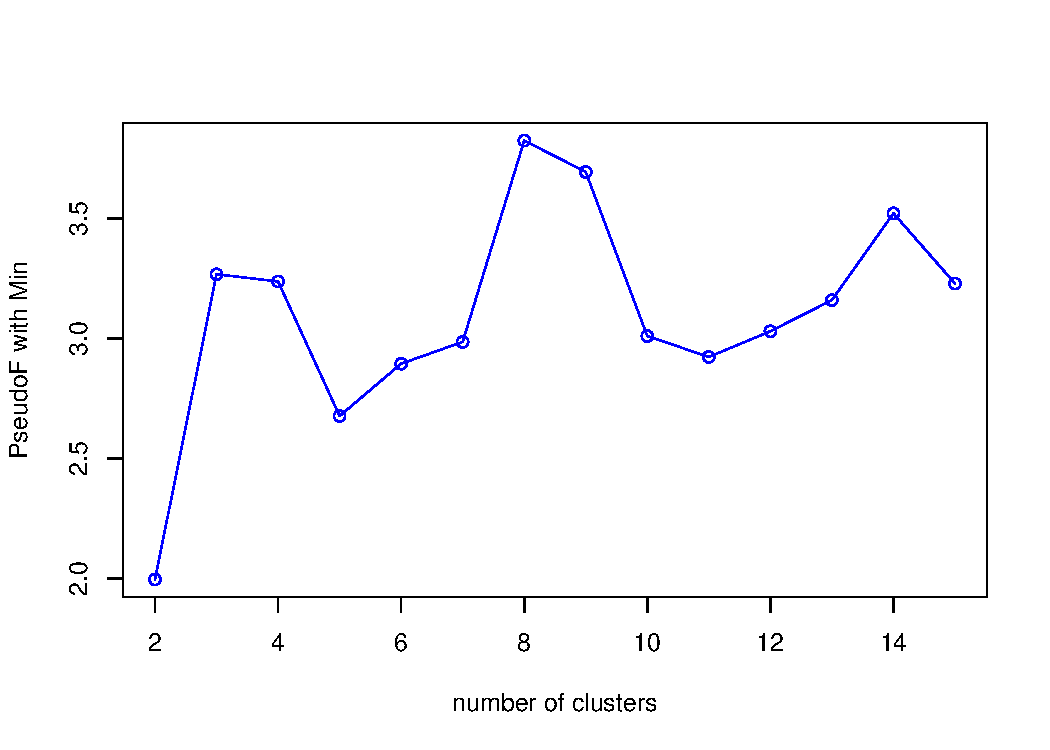
\includegraphics[width=0.45\hsize]{norm_comp-PseudoFwithMin.pdf}
}~
\subfigure[変動値のモデルパラメータの標準化後の主成分]{
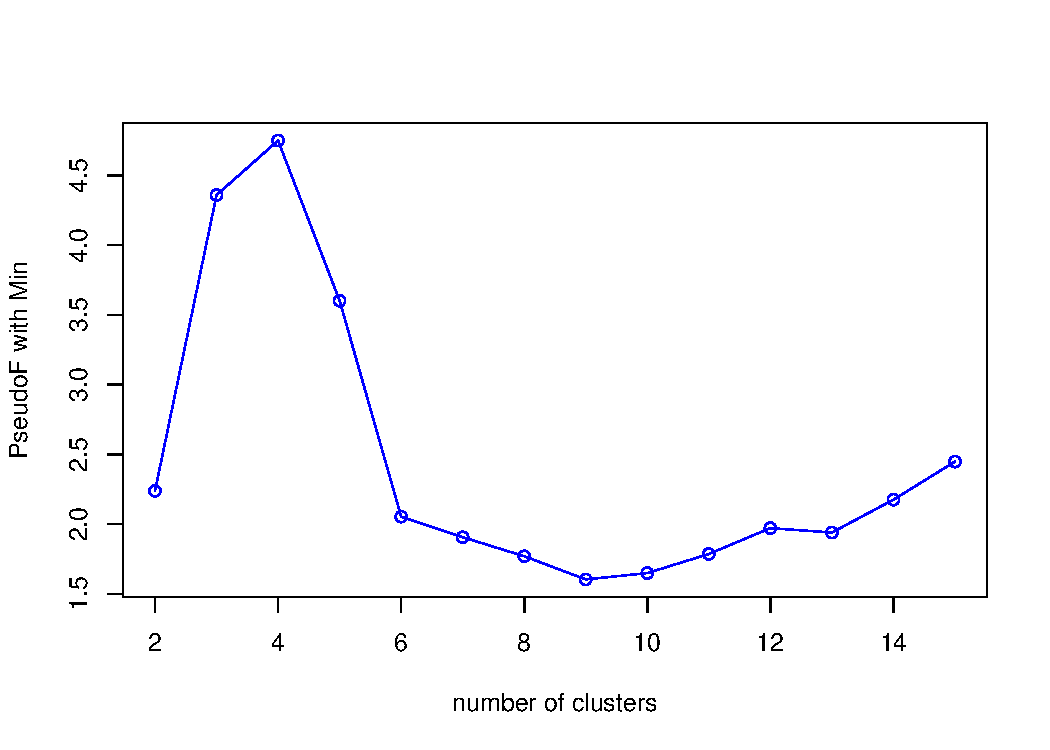
\includegraphics[width=0.45\hsize]{diff_comp-PseudoFwithMin.pdf}
}
\caption{クラスタ数と Pseudo F with Min の関係}
\label{PseudoFwithMinPlot}
\end{center}
\end{figure}

このもとでクラスタリングを行った結果を図 \ref{norm} と図 \ref{diff} に示す.
横軸に示すそれぞれのクラスタについて,各時間帯の区間データ数とその占める割合をそれぞれ図 (a)と図 (c) に示し,また各曜日の区間データ数とその区間データが占める割合をそれぞれ図 (b) と図 (d) に積み上げグラフで示している.
また,図 (e) では,横軸を曜日ごと,さらに時間帯で区切り,各クラスタに属する区間データの割合を積み上げグラフで示している.
各曜日,時間帯の区間データ数を上部に示す.

\begin{figure}[tb]
\begin{center}
\subfigure[時間帯での分類(区間データ数)]{
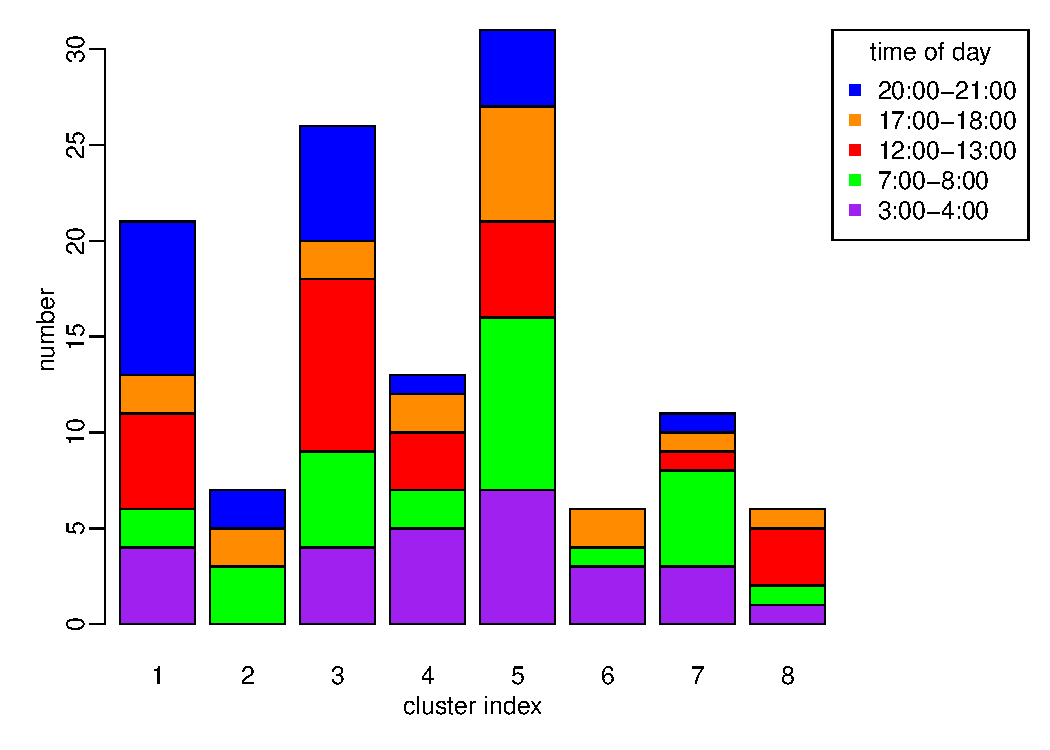
\includegraphics[width=0.45\hsize]{num-norm_comp-eucl-ward-8-timezone.pdf}
}~
\subfigure[曜日での分類(区間データ数)]{
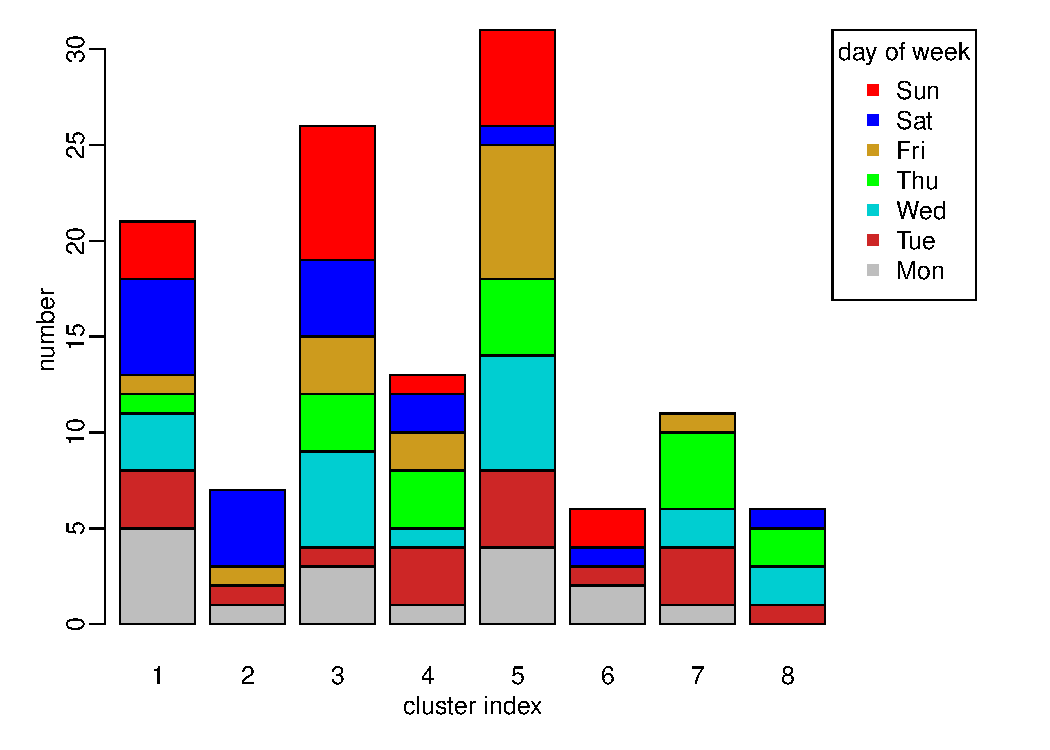
\includegraphics[width=0.45\hsize]{num-norm_comp-eucl-ward-8-day.pdf}
}\\
\subfigure[時間帯での分類(割合)]{
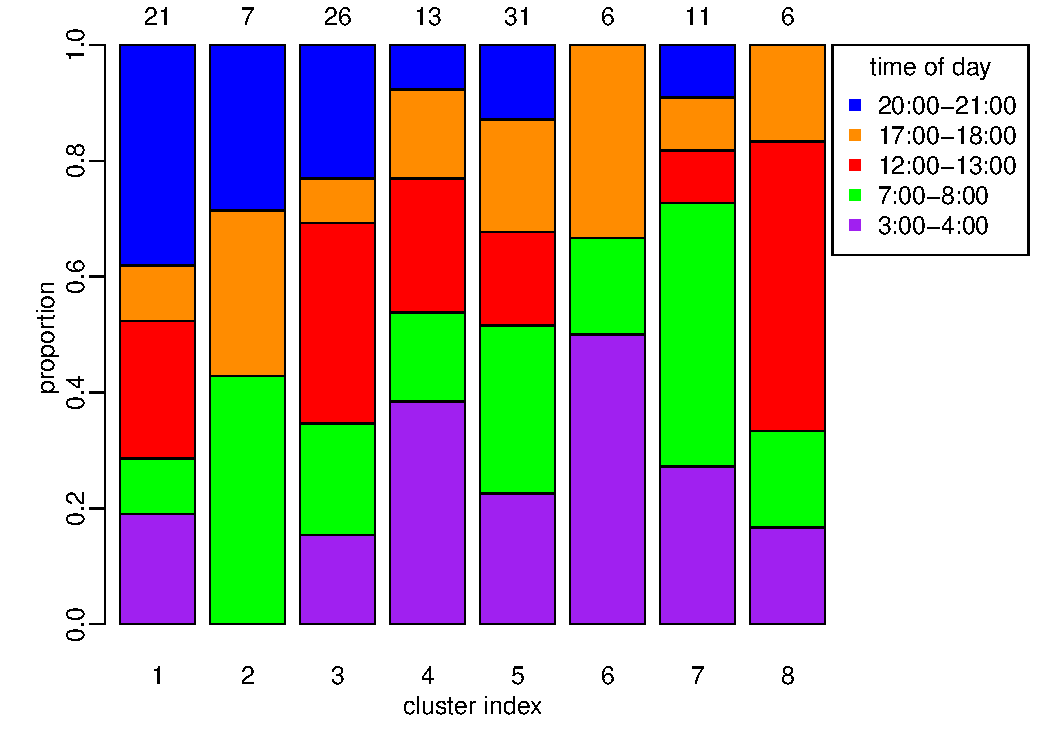
\includegraphics[width=0.45\hsize]{norm_comp-eucl-ward-8-timezone.pdf}
}~
\subfigure[曜日での分類(割合)]{
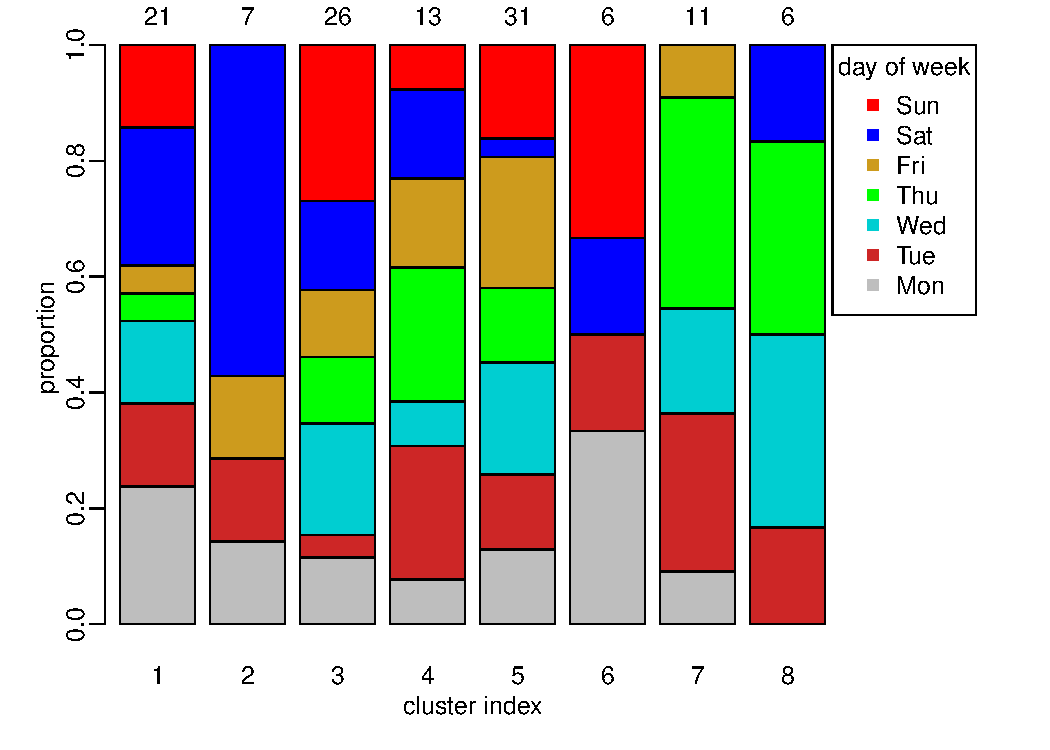
\includegraphics[width=0.45\hsize]{norm_comp-eucl-ward-8-day.pdf}
}\\
\subfigure[時間帯と曜日での分類(割合)]{
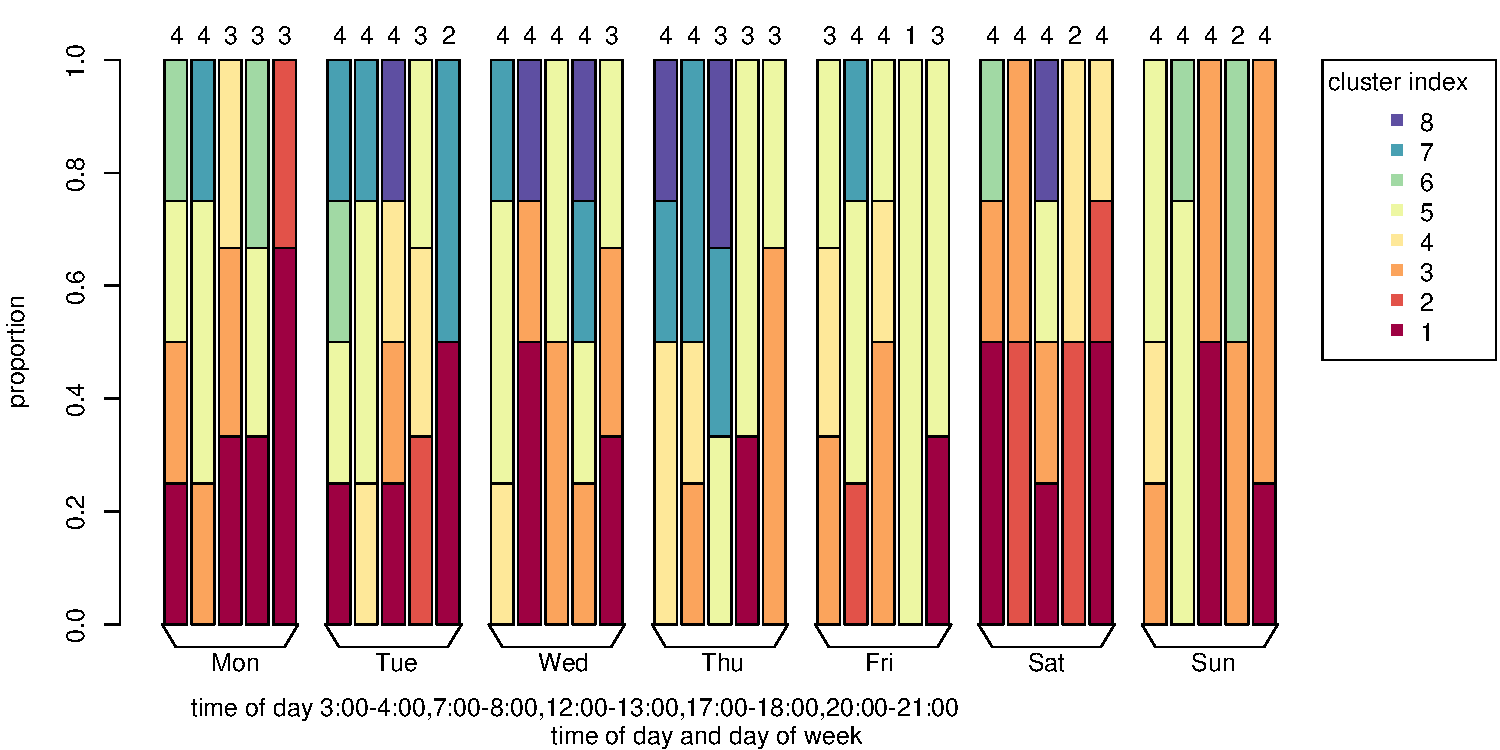
\includegraphics[width=0.8\hsize]{norm_comp-eucl-ward-8-timezone-day.pdf}
}
\caption{実測値のモデルパラメータの標準化後の主成分によるクラスタリング結果}
\label{norm}
\end{center}
\end{figure}

\begin{figure}[tb]
\begin{center}
\subfigure[時間帯での分類(区間データ数)]{
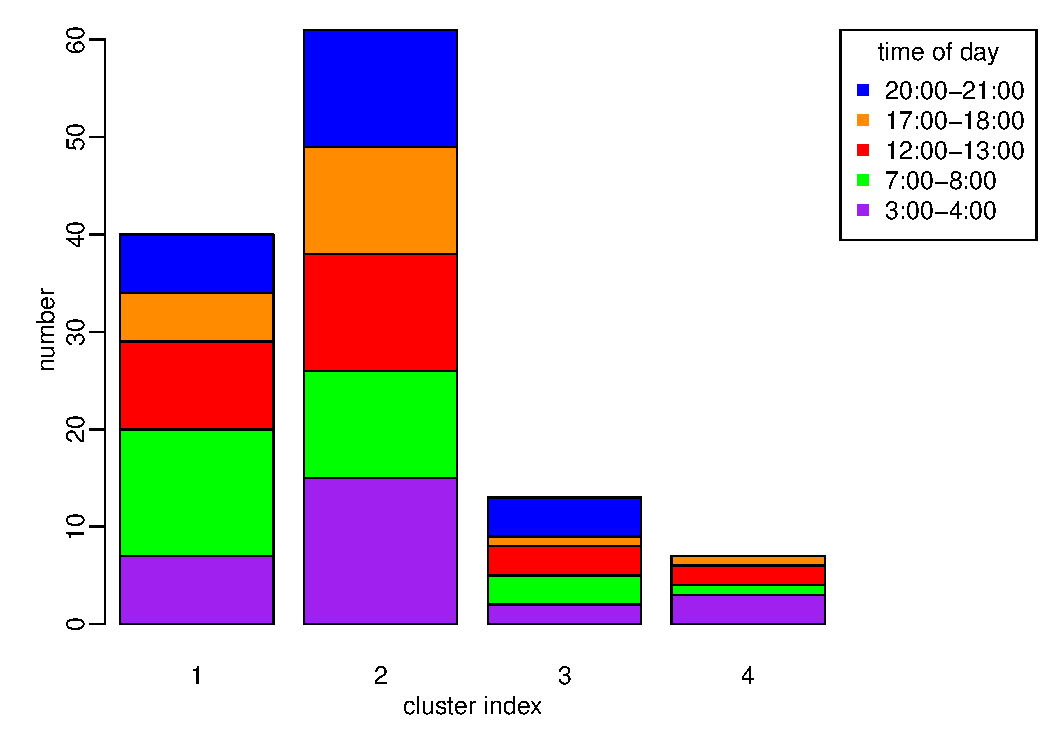
\includegraphics[width=0.45\hsize]{num-diff_comp-eucl-ward-4-timezone.pdf}
}~
\subfigure[曜日での分類(区間データ数)]{
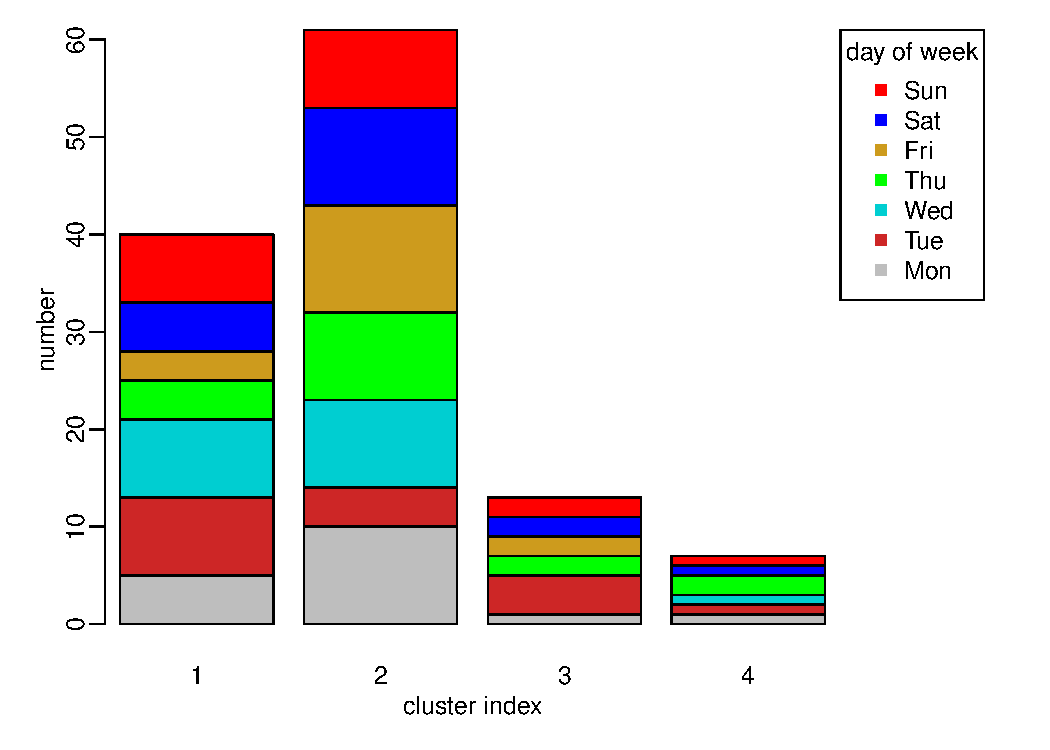
\includegraphics[width=0.45\hsize]{num-diff_comp-eucl-ward-4-day.pdf}
}\\
\subfigure[時間帯での分類(割合)]{
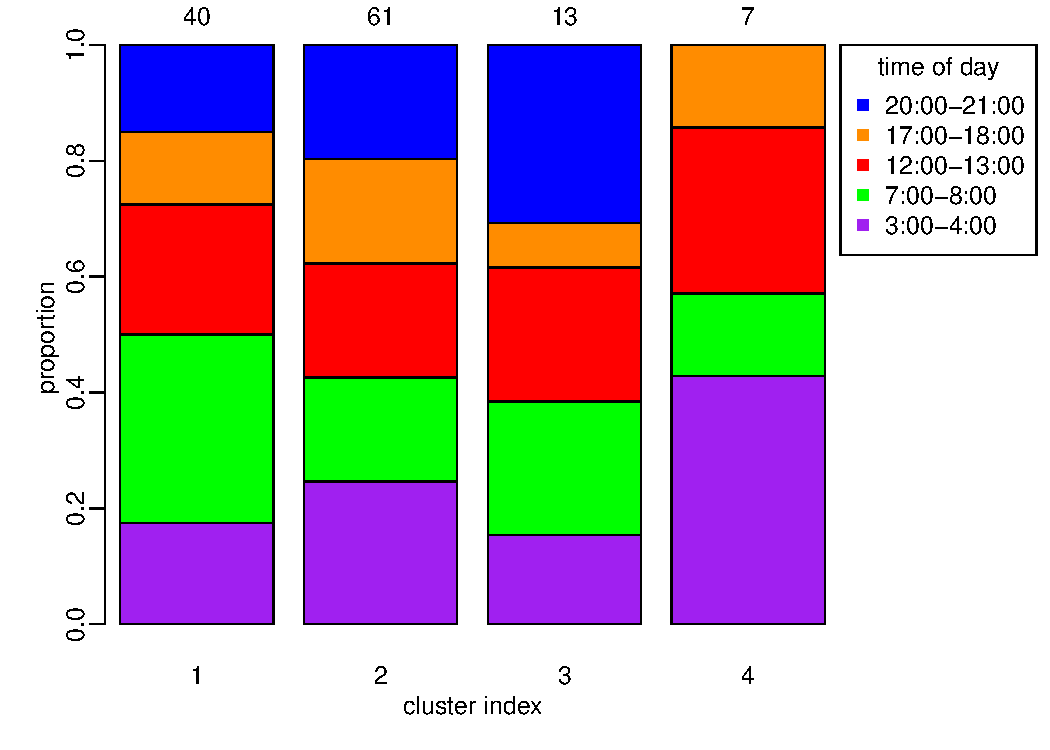
\includegraphics[width=0.45\hsize]{diff_comp-eucl-ward-4-timezone.pdf}
}~
\subfigure[曜日での分類(割合)]{
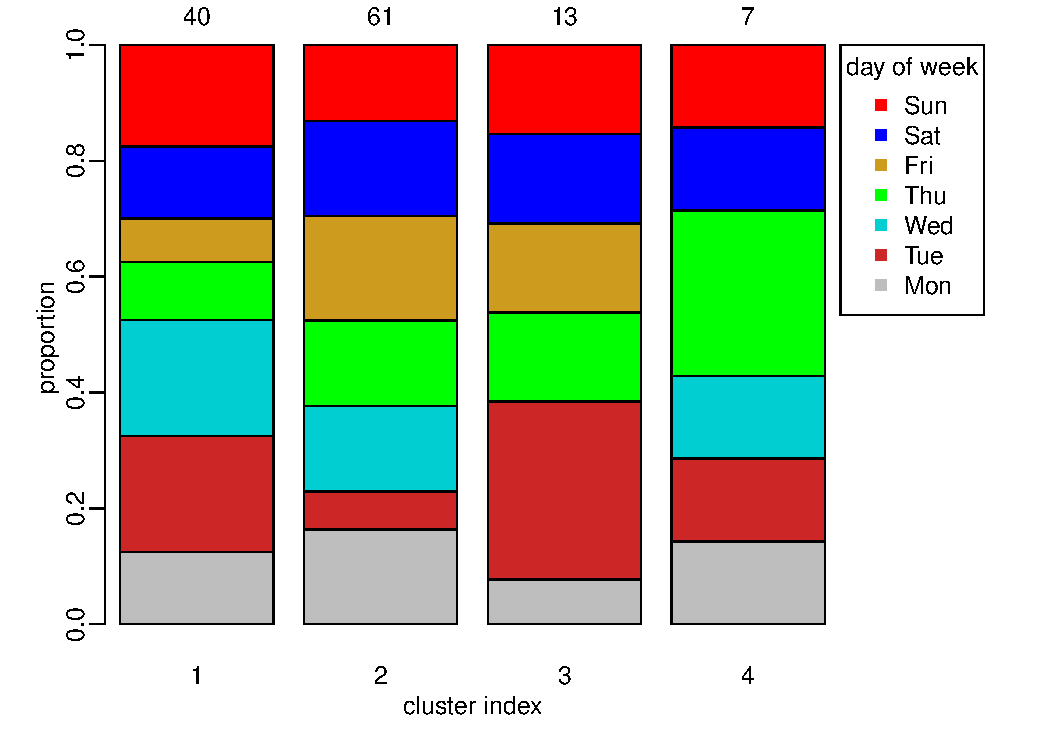
\includegraphics[width=0.45\hsize]{diff_comp-eucl-ward-4-day.pdf}
}\\
\subfigure[時間帯と曜日での分類(割合)]{
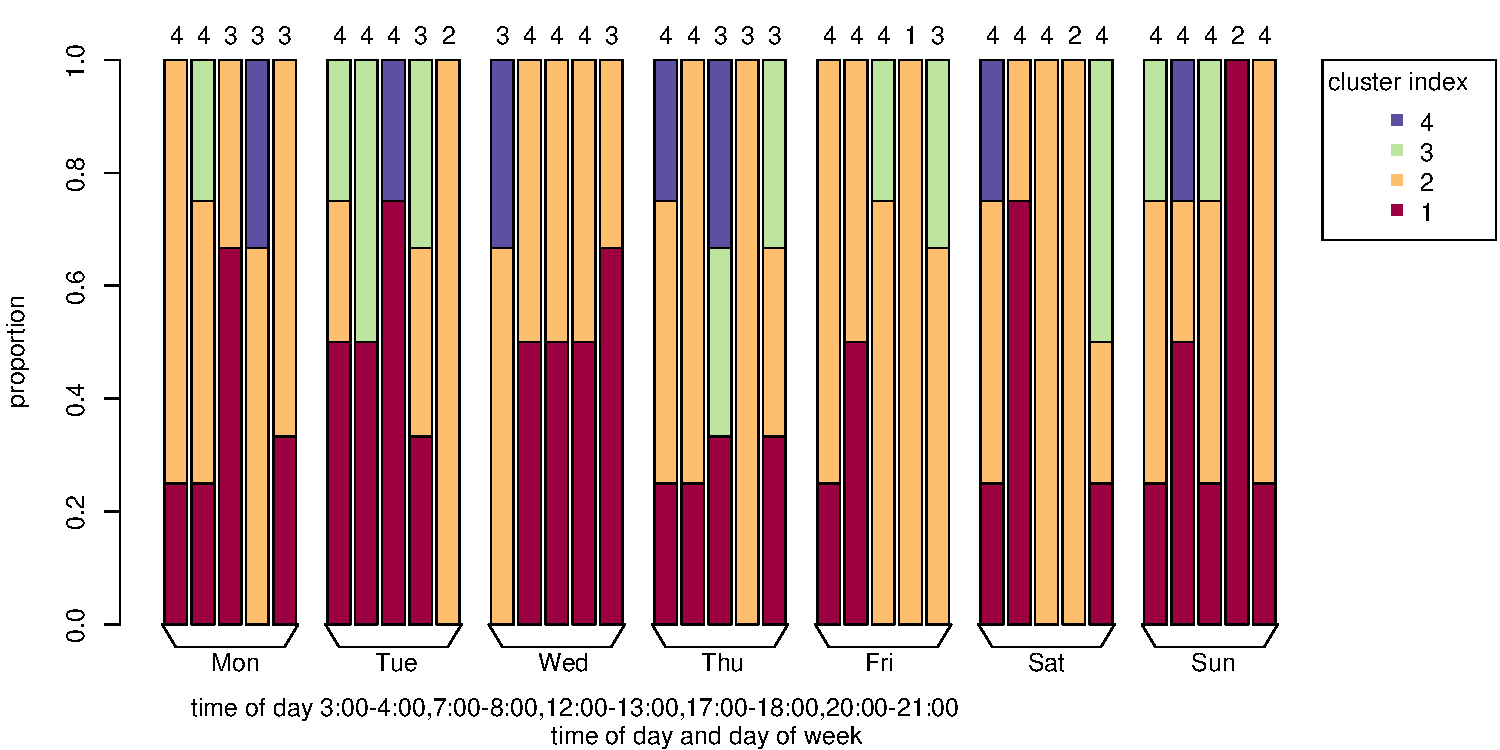
\includegraphics[width=0.8\hsize]{diff_comp-eucl-ward-4-timezone-day.pdf}
}
\caption{変動値のモデルパラメータの標準化後の主成分によるクラスタリング結果}
\label{diff}
\end{center}
\end{figure}

図 \ref{norm}(a),(c) より,いずれのクラスタにおいてもすべての時間帯の区間データが一様に含まれているということはなく,属する区間データには時間帯による偏りがあることがわかる.
これらの偏りは,我が国の移動通信トラヒックが関係していると考えられる(図 \ref{traffic})\cite{soumutrafficstatics}.
\begin{figure}[tb]
\centering
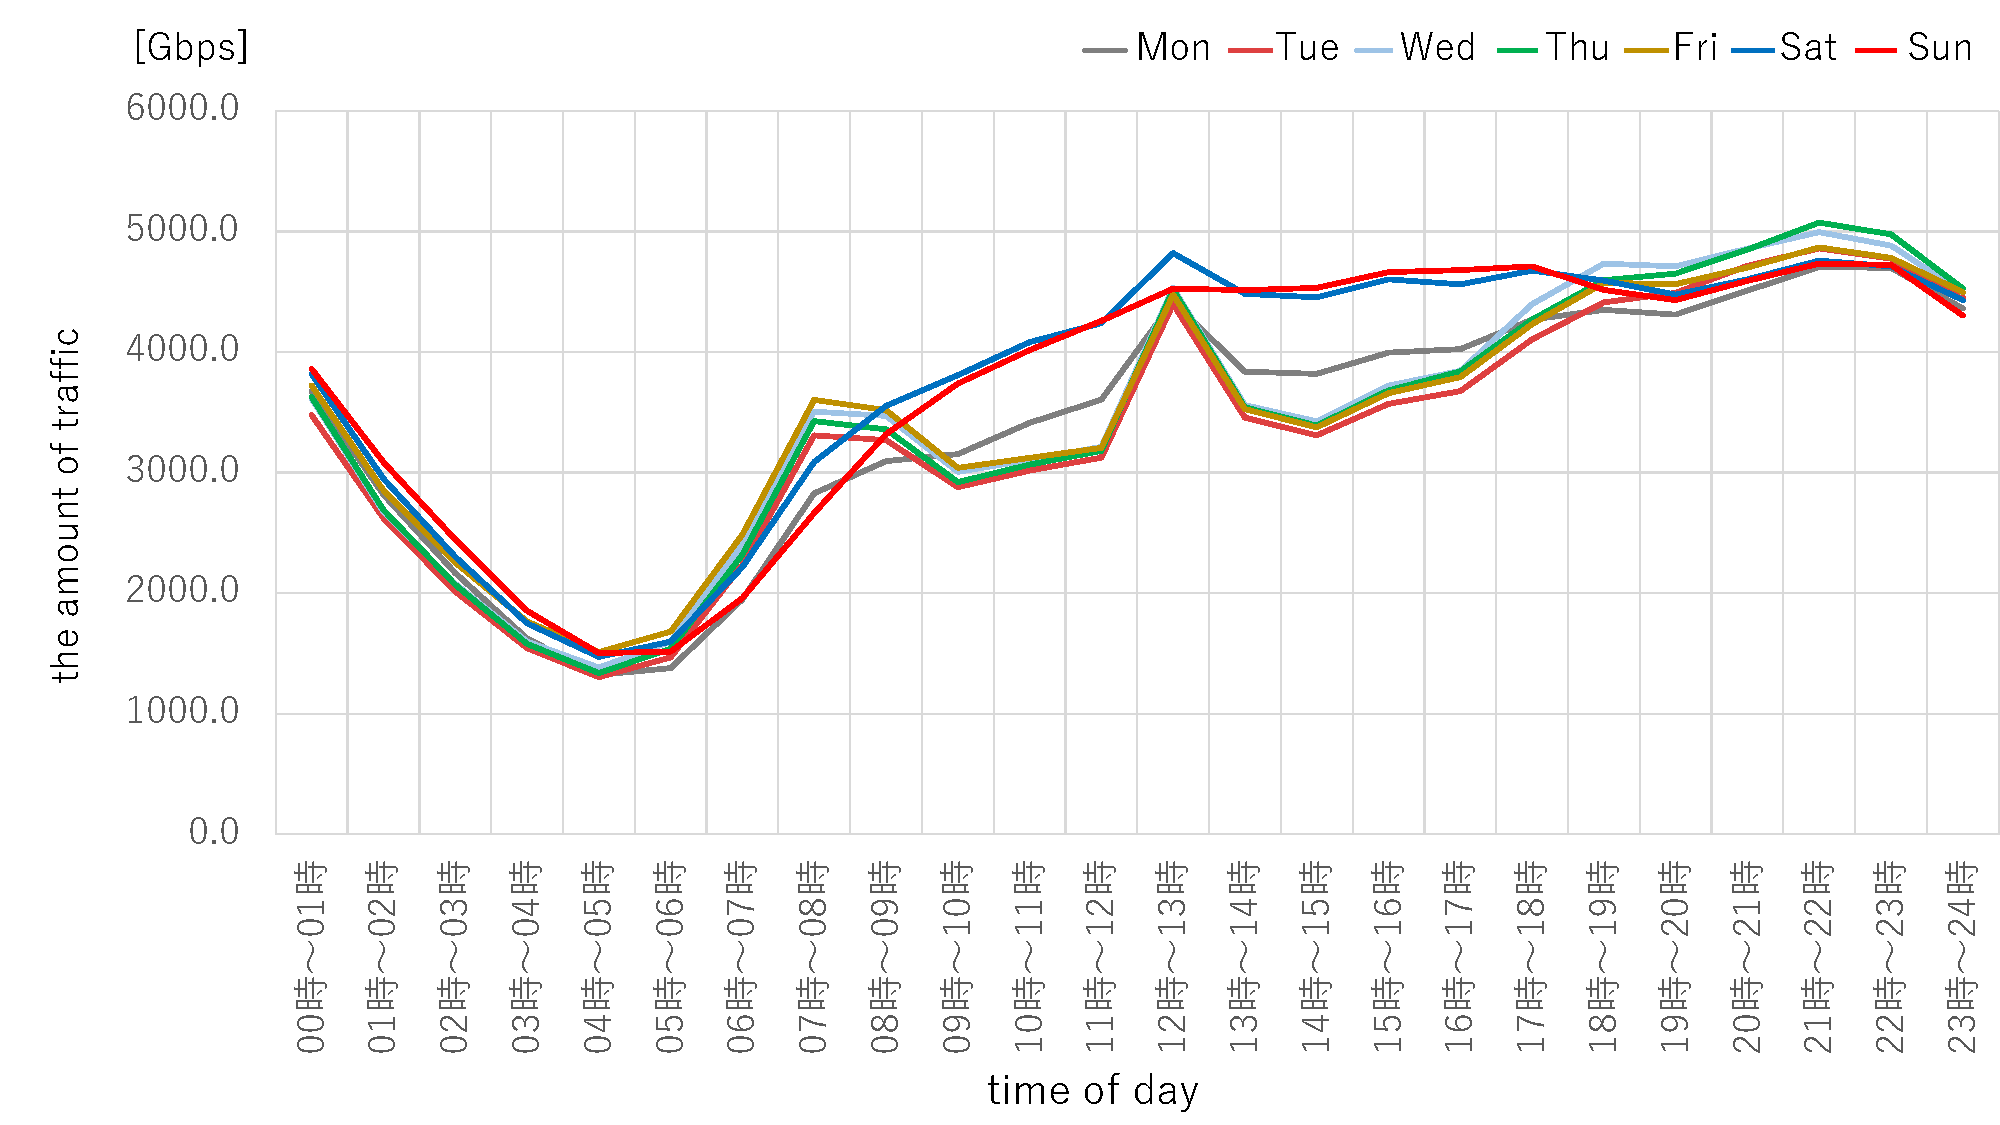
\includegraphics[width=0.8\hsize]{traffic.pdf}
\caption{曜日ごとの時間帯と平均移動通信トラヒック量の関係}
\label{traffic}
\end{figure}

\subsection{主成分分析なしでのクラスタリング}
ここでは,クラスタリングパラメータの前処理として式 (\ref{scale}) で表される標準化のみを行いその後の主成分分析は行わものとする.
 
クラスタ数は式 (\ref{PseudoFwithMin}) で表される PseudoF with Min を用いて定量的に定める.
実測値および変動値のそれぞれのモデルパラメータに対して標準化を行って得られるパラメータを用いて,クラスタ数を変えながら Pseudo F with Min を求めた結果を図 \ref{PseudoFwithMinPlotScale} に示す.図より,実測値の場合にはクラスタ数 11 で,変動値の場合にはクラスタ数 3 でそれぞれ Pseudo F with Min が最大になることがわかる.
\begin{figure}[tb]
\begin{center}
\subfigure[標準化した実測値のモデルパラメータ]{
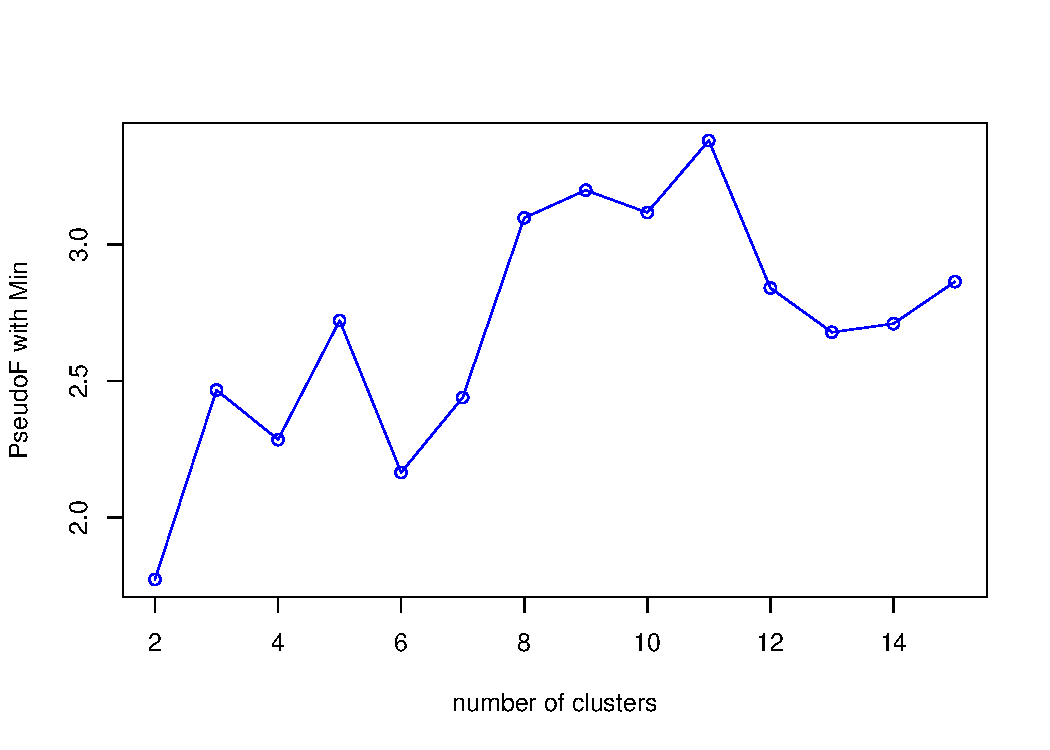
\includegraphics[width=0.45\hsize]{norm_scale-PseudoFwithMin.pdf}
}~
\subfigure[標準化した変動値のモデルパラメータ]{
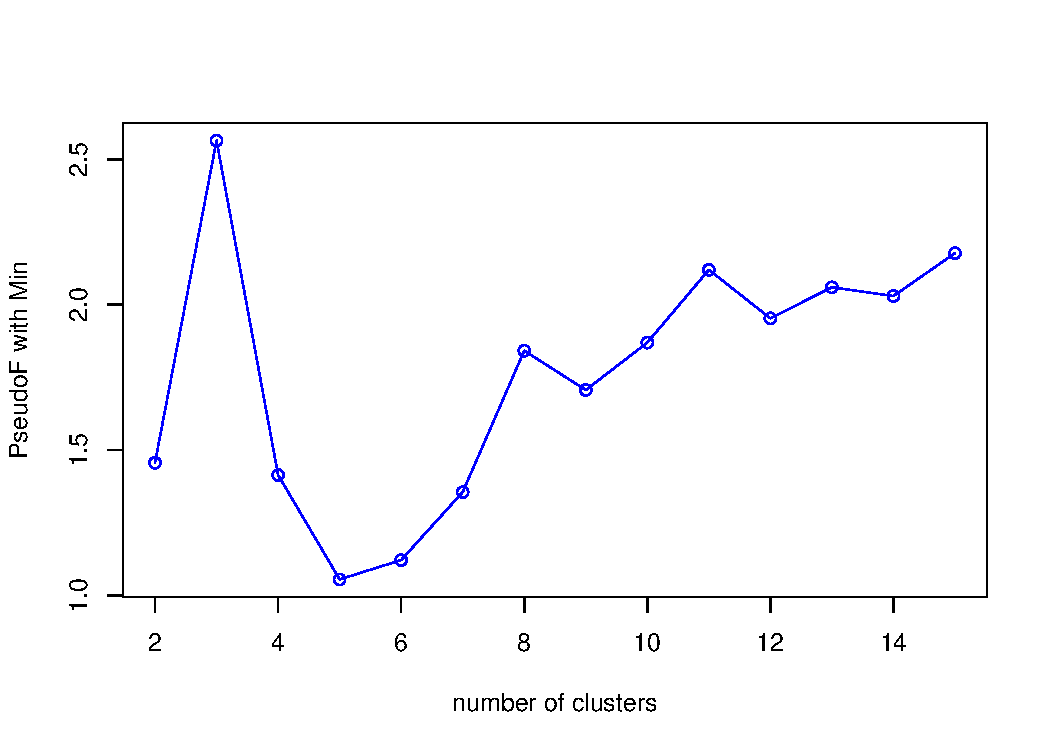
\includegraphics[width=0.45\hsize]{diff_scale-PseudoFwithMin.pdf}
}
\caption{クラスタ数と Pseudo F with Min の関係}
\label{PseudoFwithMinPlotScale}
\end{center}
\end{figure} 

このもとでクラスタリングを行った結果を図 \ref{normScale} と図 \ref{diffScale} に示す.
横軸に示すそれぞれのクラスタについて,各時間帯の区間データ数とその占める割合をそれぞれ図 (a)と図 (c) に示し,また各曜日の区間データ数とその区間データが占める割合をそれぞれ図 (b) と図 (d) に積み上げグラフで示している.
また,図 (e) では,横軸を曜日ごと,さらに時間帯で区切り,各クラスタに属する区間データの割合を積み上げグラフで示している.
各曜日,時間帯の区間データ数を上部に示す.

\begin{figure}[tb]
\begin{center}
\subfigure[時間帯での分類(区間データ数)]{
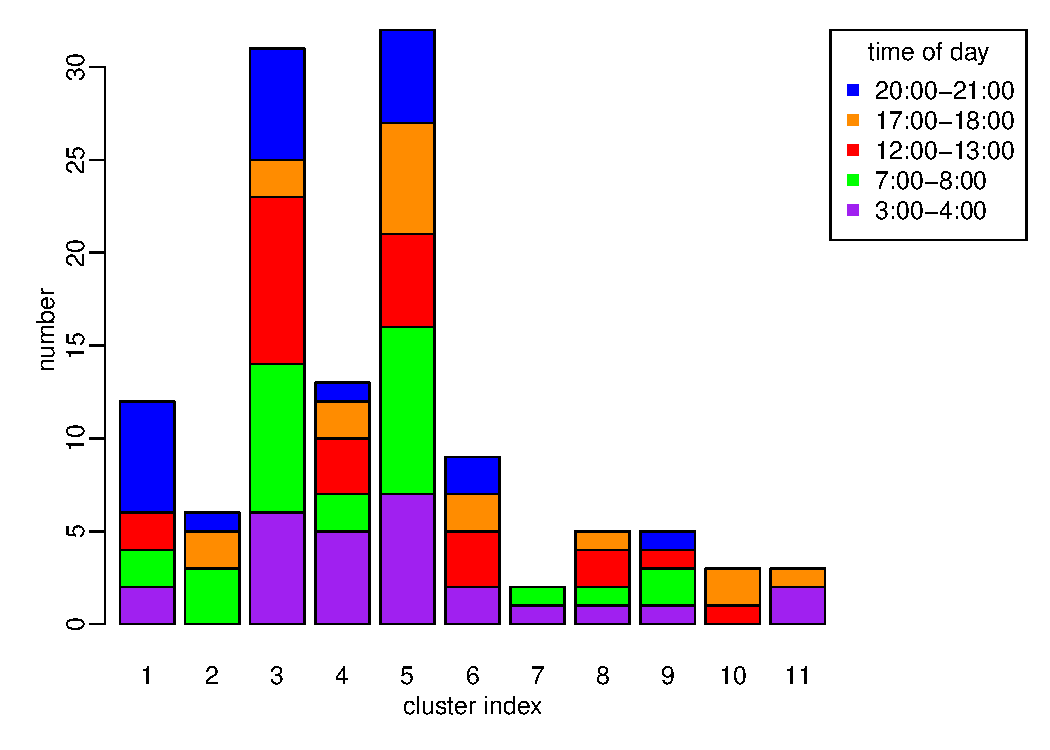
\includegraphics[width=0.45\hsize]{num-norm_scale-eucl-ward-11-timezone.pdf}
}~
\subfigure[曜日での分類(区間データ数)]{
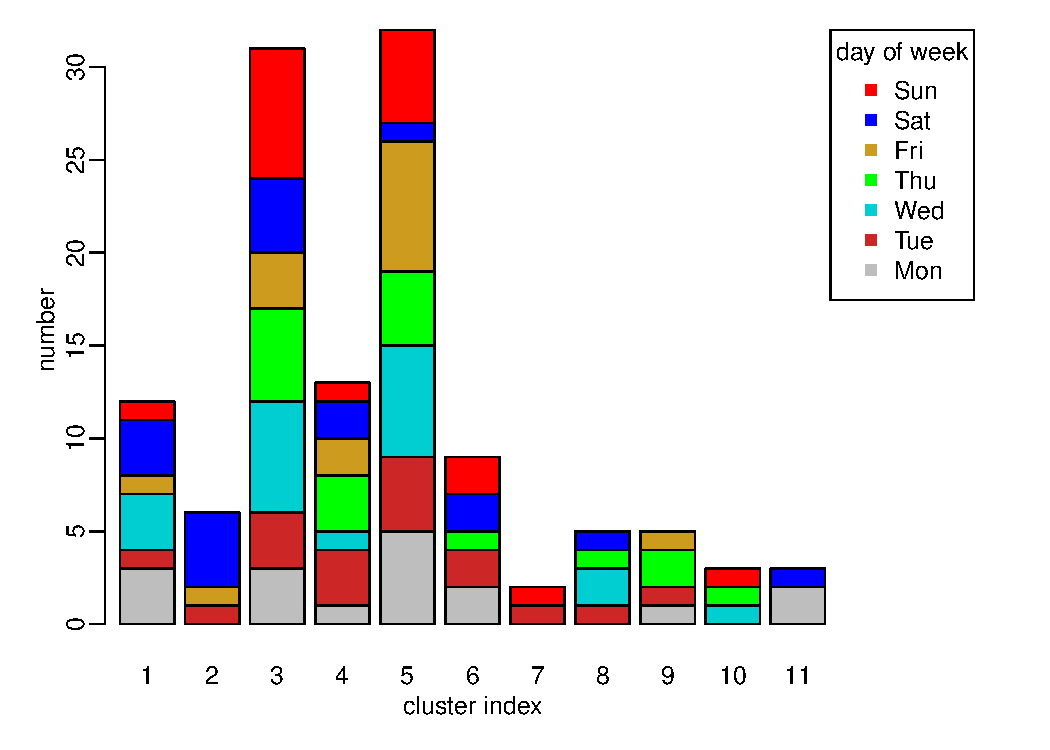
\includegraphics[width=0.45\hsize]{num-norm_scale-eucl-ward-11-day.pdf}
}\\
\subfigure[時間帯での分類(割合)]{
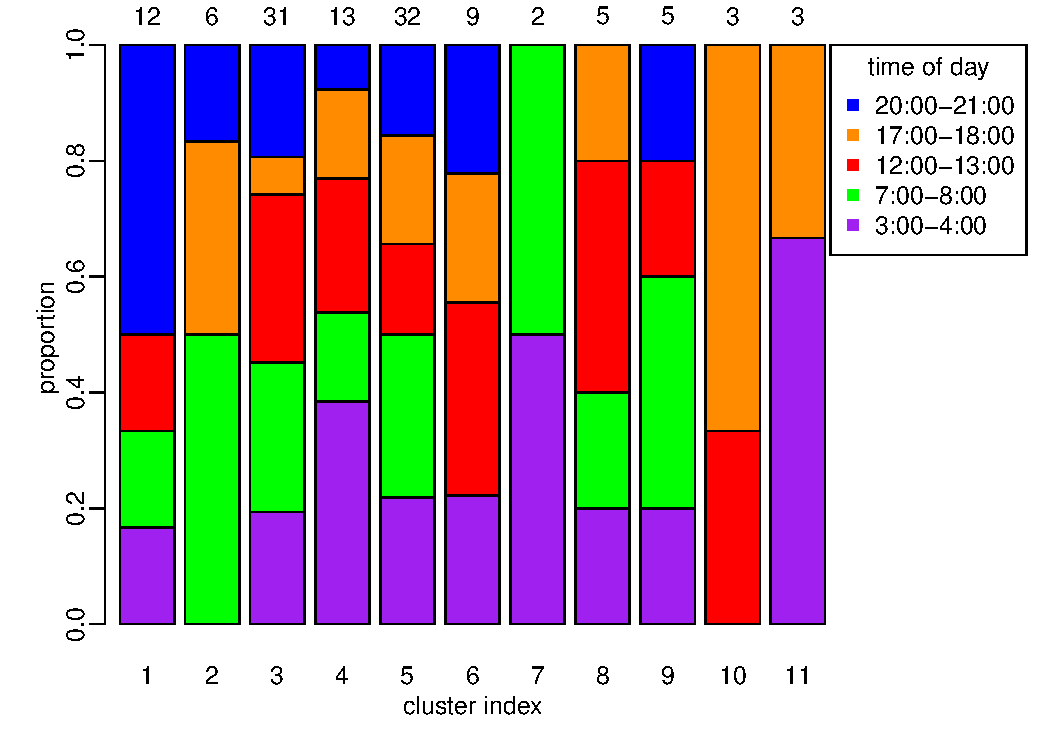
\includegraphics[width=0.45\hsize]{norm_scale-eucl-ward-11-timezone.pdf}
}~
\subfigure[曜日での分類(割合)]{
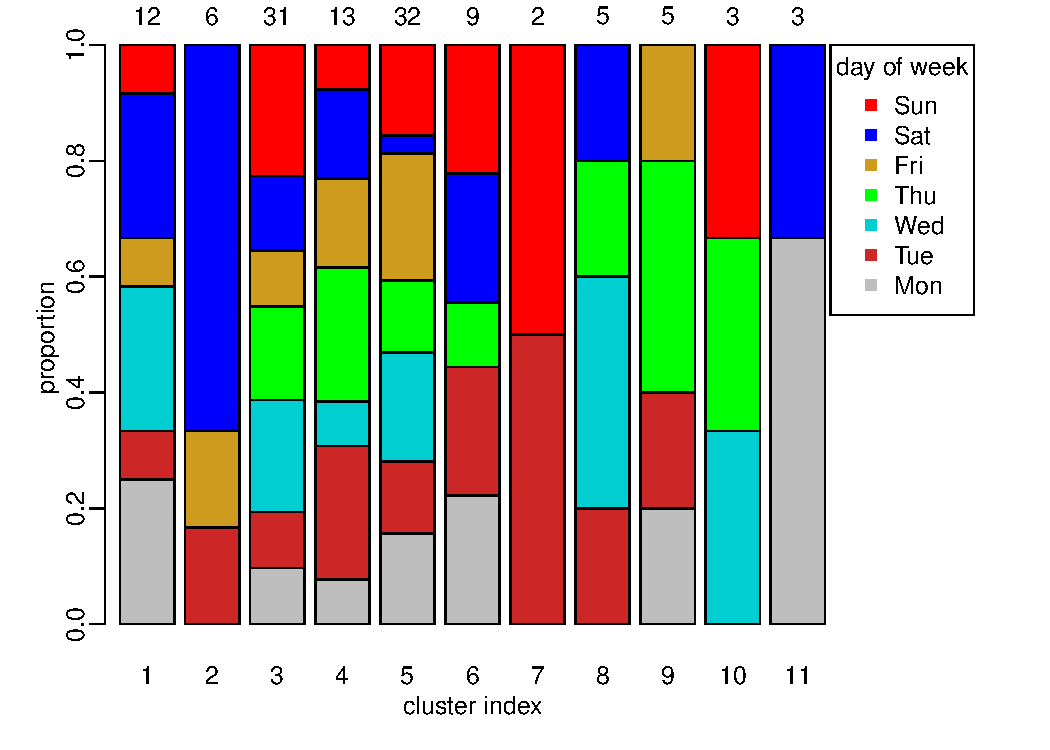
\includegraphics[width=0.45\hsize]{norm_scale-eucl-ward-11-day.pdf}
}\\
\subfigure[時間帯と曜日での分類(割合)]{
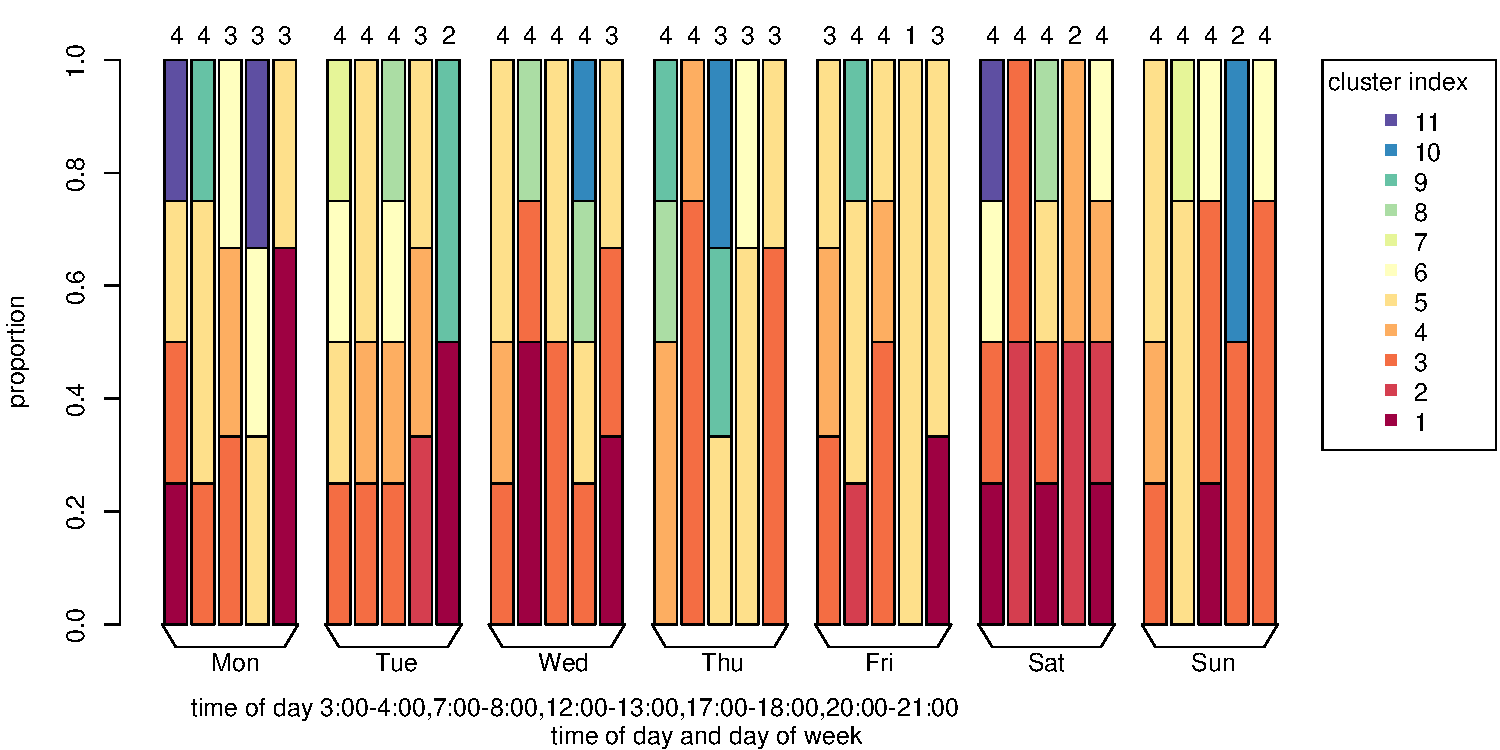
\includegraphics[width=0.8\hsize]{norm_scale-eucl-ward-11-timezone-day.pdf}
}
\caption{実測値のモデルパラメータの標準化によるクラスタリング結果}
\label{normScale}
\end{center}
\end{figure}

\begin{figure}[tb]
\begin{center}
\subfigure[時間帯での分類(区間データ数)]{
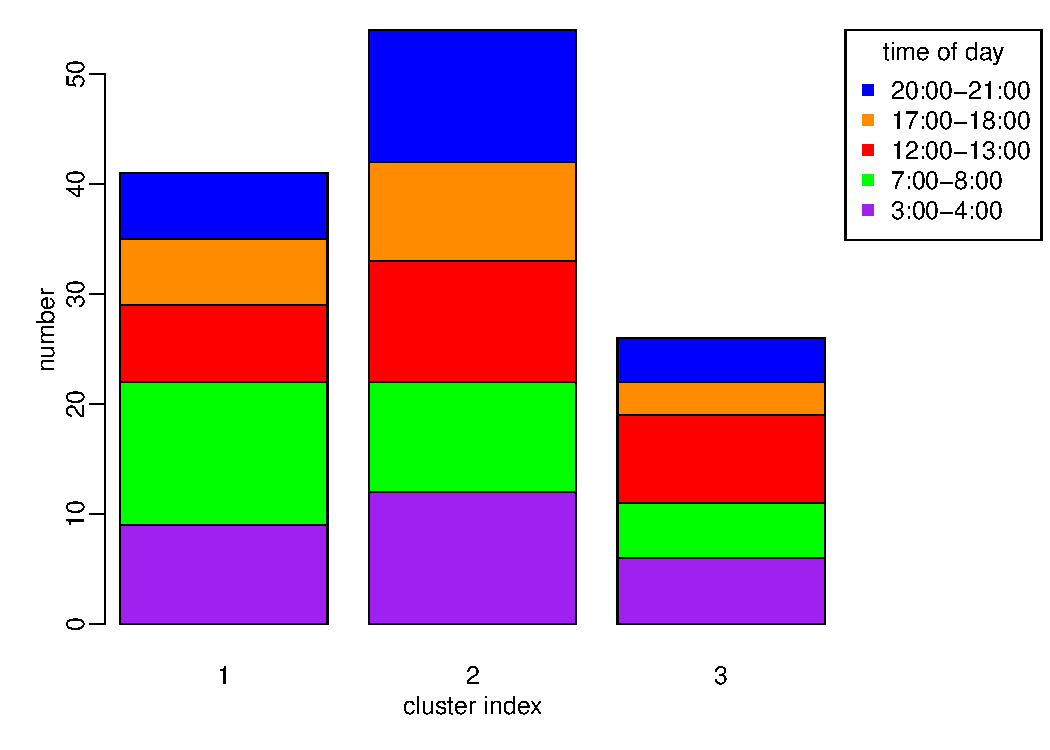
\includegraphics[width=0.45\hsize]{num-diff_scale-eucl-ward-3-timezone.pdf}
}~
\subfigure[曜日での分類(区間データ数)]{
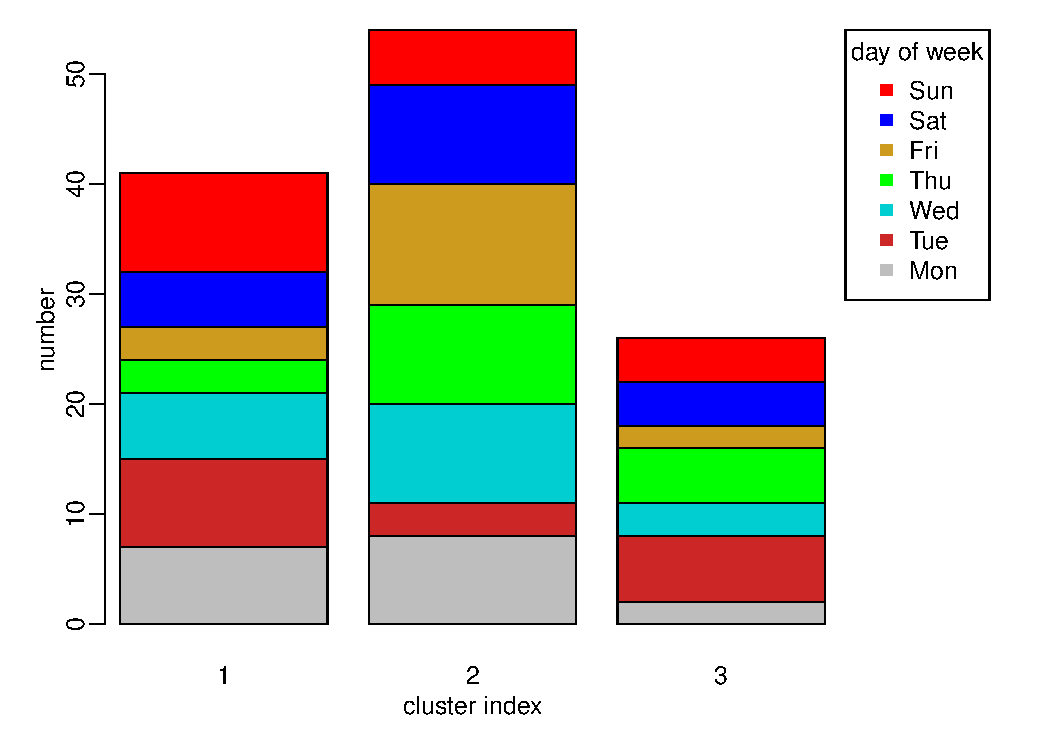
\includegraphics[width=0.45\hsize]{num-diff_scale-eucl-ward-3-day.pdf}
}\\
\subfigure[時間帯での分類(割合)]{
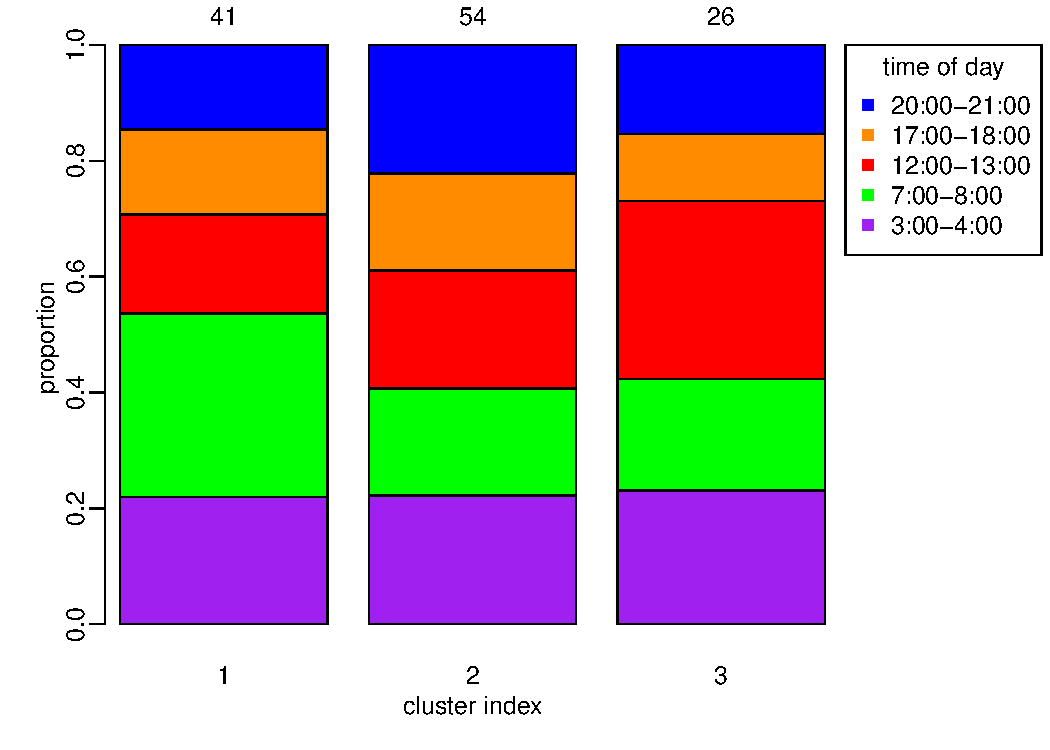
\includegraphics[width=0.45\hsize]{diff_scale-eucl-ward-3-timezone.pdf}
}~
\subfigure[曜日での分類(割合)]{
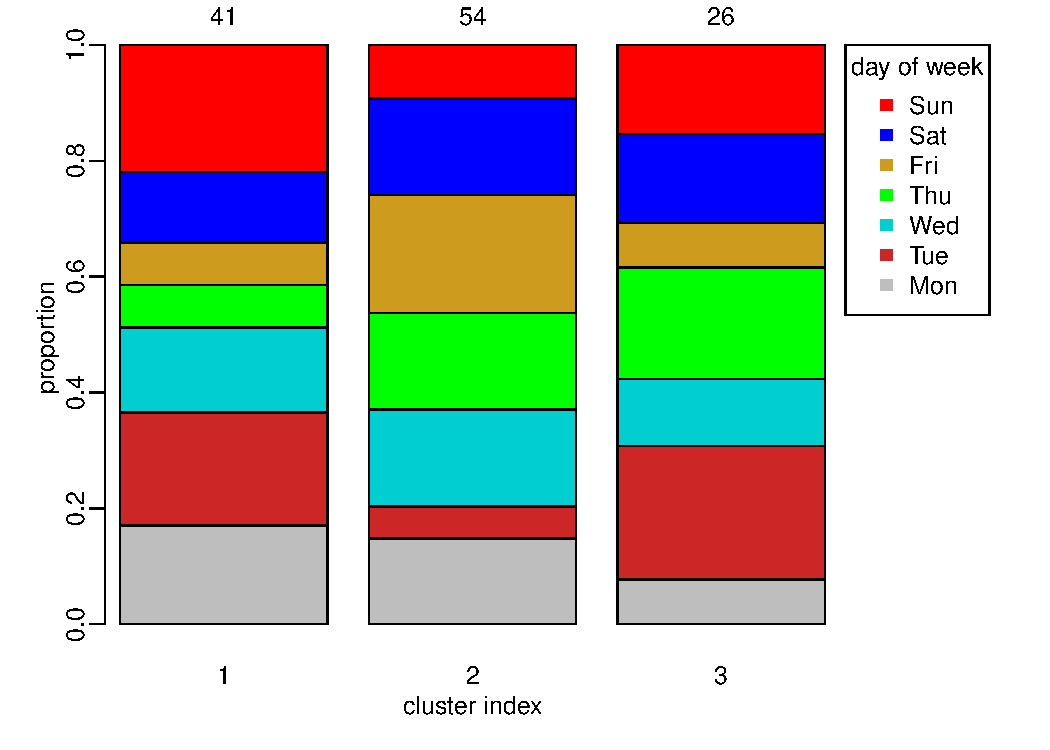
\includegraphics[width=0.45\hsize]{diff_scale-eucl-ward-3-day.pdf}
}\\
\subfigure[時間帯と曜日での分類(割合)]{
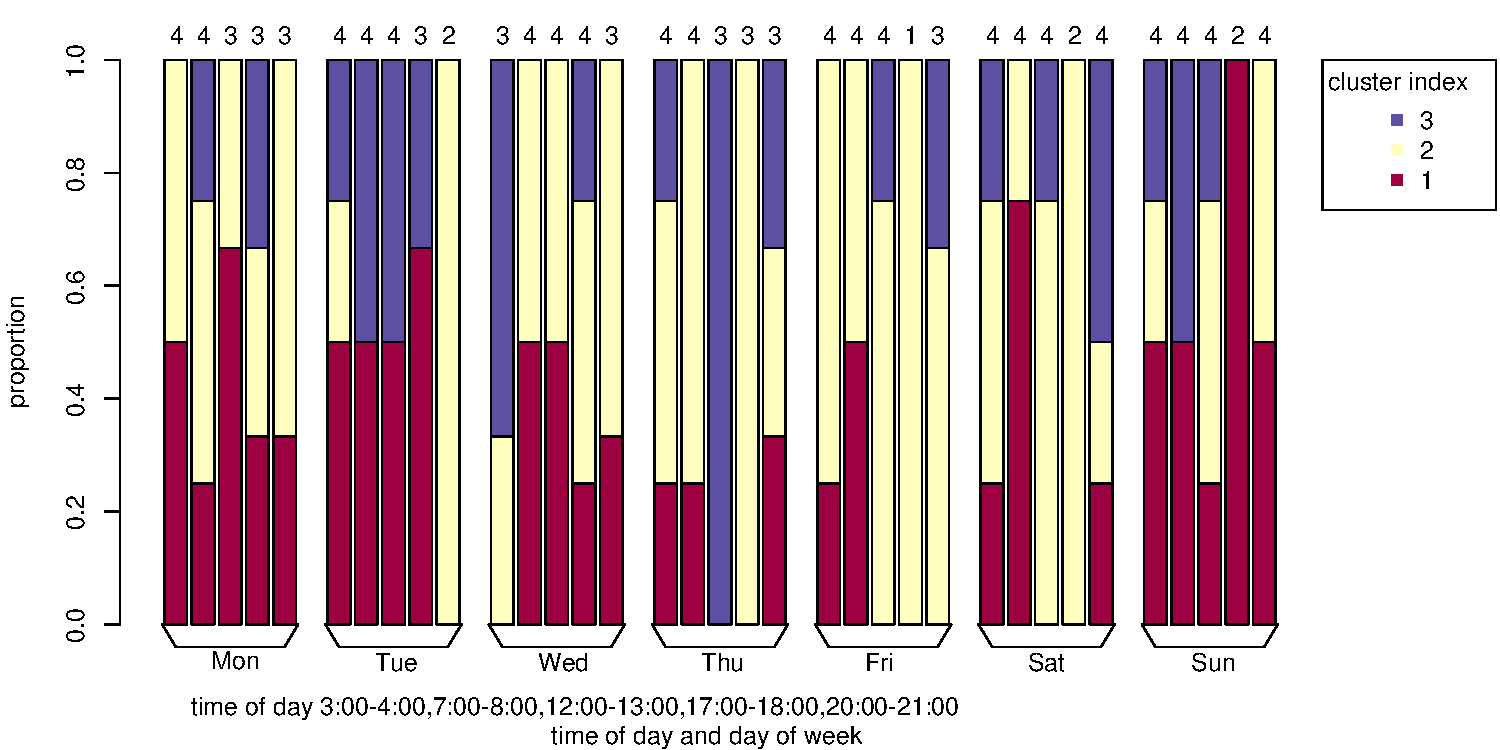
\includegraphics[width=0.8\hsize]{diff_scale-eucl-ward-3-timezone-day.pdf}
}
\caption{変動値のモデルパラメータの標準化によるクラスタリング結果}
\label{diffScale}
\end{center}
\end{figure}

まず,実測値の場合は図 \ref{normScale} のように計 11 個のクラスタが形成される.しかし,いくつかのクラスタはその要素数が少なく,時間や曜日に応じた共通の傾向を見出すことが困難であった.そこでここでは,要素数が 10 を超えるクラスタ 1,クラスタ 3,クラスタ 4,クラスタ 5 にのみ注目した.
結果としては,IN 研究会での発表と同様の傾向が見られた.
具体的には,クラスタ 1 とクラスタ 3 には,図 (\ref{normScale}-b)と 図(\ref{normScale}-d) より,一日を通じて移動通信トラヒックが多い土日の計測データが多く属しており,クラスタ 1 には 20 時台,クラスタ 3 には 12 時台とそれぞれ移動通信トラキック量が多い時間帯の計測データが多く属していた.また,クラスタ 4 には移動通信トラヒックが少ない 3 時台が多く属しており,クラスタ 5 には変化の激しい平日のデータが多く属していた.
しかし,どれもクラスタ単位での議論であり,特定のクラスタに特定の時間帯や曜日がまとまって分類されるような顕著な傾向は見て取れない.

次に変動値の場合は,図 \ref{diffScale} のような 3 つのクラスタに計測データが万遍なく属する結果が得られた.ただ,わずかながらもクラスタ 1 には 7 時台,クラスタ 3 には 12 時台が多く属しているように見える.

\section{大きな応答遅延の単発性の確認}
15 秒周期で行ってきたこれまでの計測実験において,突発的にスパイク状の応答遅延が発生することが確認されている.
そこでここでは,それが本当に単発的なのか,あるいは 15 秒よりも短い計測周期なら連続して得られるのかを調べる.
これには,ping を用いた応答遅延の計測間隔をできるだけ小さくする方法をとる.
具体的には,Raspberry Pi 上で 15 秒毎に,時刻取得後に AWS サーバ(13.231.224.193)に対して ping (パケットサイズ 60 バイト, ICMP ECHO メッセージ,パケット数 1)を用いた応答遅延の計測を 10 ミリ秒間隔で計 10 回行う python スクリプトを 2 時間に渡って実行した.
計測は 6 月 24 日 の 12:00 から 14:00 までとし,Raspberry Pi は若宮研究室内に設置した.
また,取得した時刻と実際に ping コマンドを実行した時刻には僅かながらのタイムラグが生じていると考えられるが,ここではそれを無視し取得した時刻に ping コマンドが実行されたものとみなす.
このようにして得られた応答遅延の ping の実行時刻を早いものから順に $t = 1,2,\ldots,4790$ として横軸に取り,縦軸に計測値を取ったグラフを図 \ref{1} と 図 \ref{2} に分けて示す.図 \ref{1} は計測開始から一時間経過後までであり,図 \ref{2} は一時間経過後から計測終了までである.また,横軸に垂直な黒色の直線によって応答遅延データは 10 個ずつの組に分けており,同一組の隣り合う計測値の時刻間隔は 10 ミリ秒であり,隣り合う組の時刻間隔は約 15 秒である.
\begin{figure}[tb]
\begin{center}
\subfigure[$0 \sim 5$分後]{
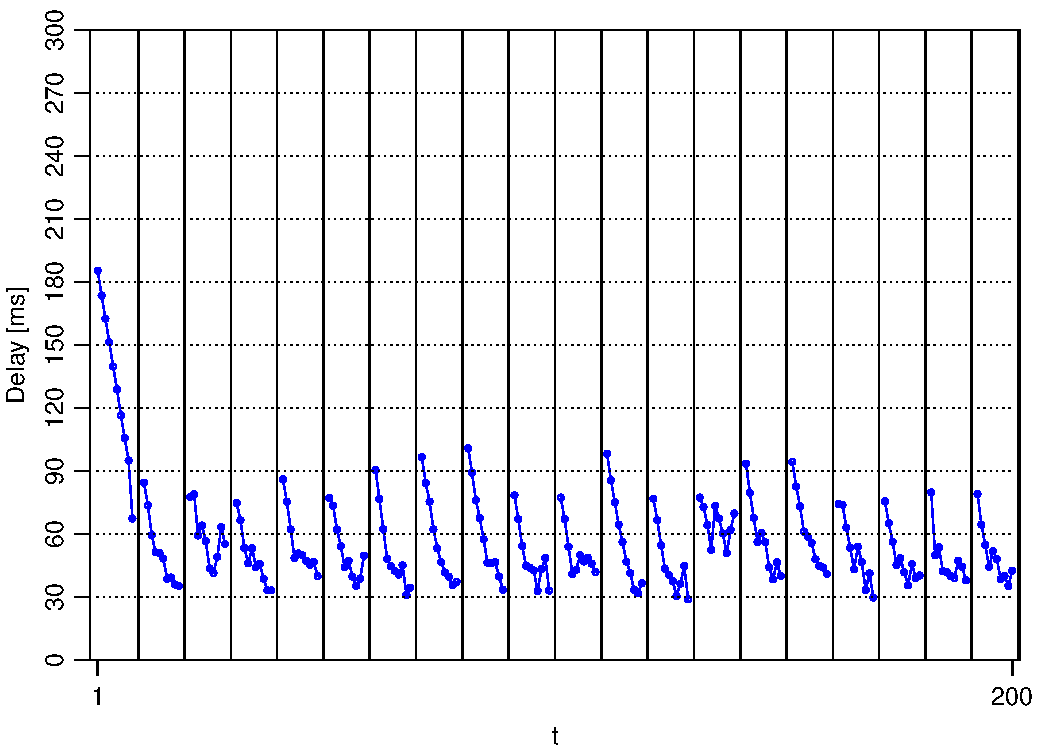
\includegraphics[width=0.33\hsize]{0-5.pdf}
}~
\subfigure[$5 \sim 10$分後]{
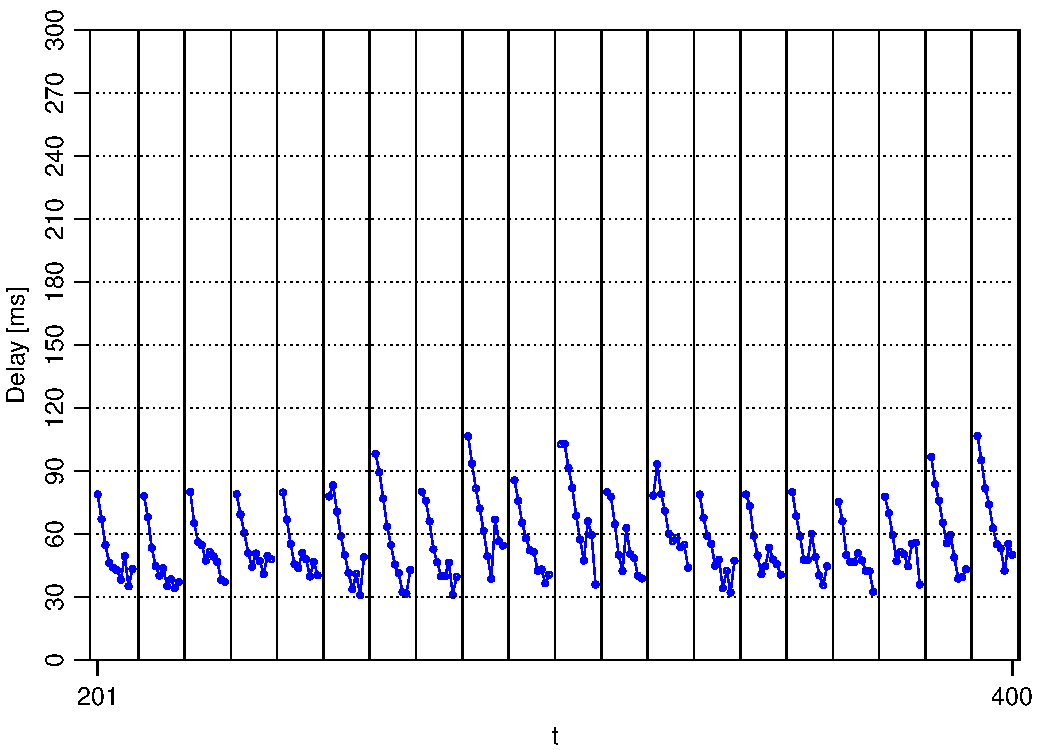
\includegraphics[width=0.33\hsize]{5-10.pdf}
}~
\subfigure[$10 \sim 15$分後]{
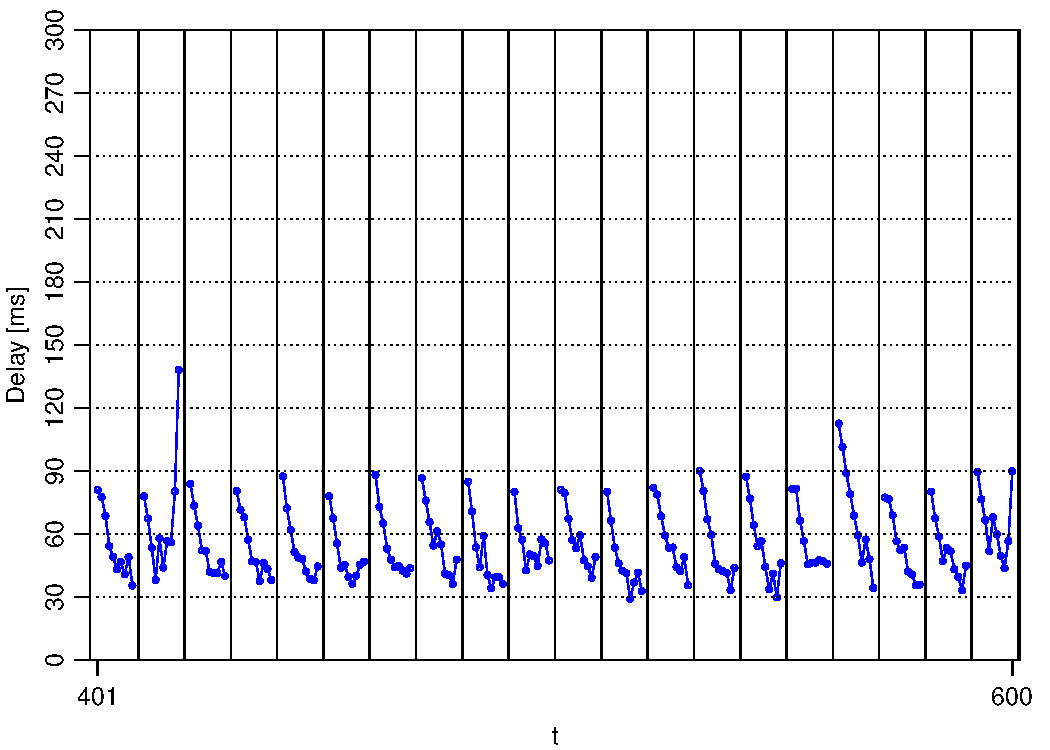
\includegraphics[width=0.33\hsize]{10-15.pdf}
}\\
\subfigure[$15 \sim 20$分後]{
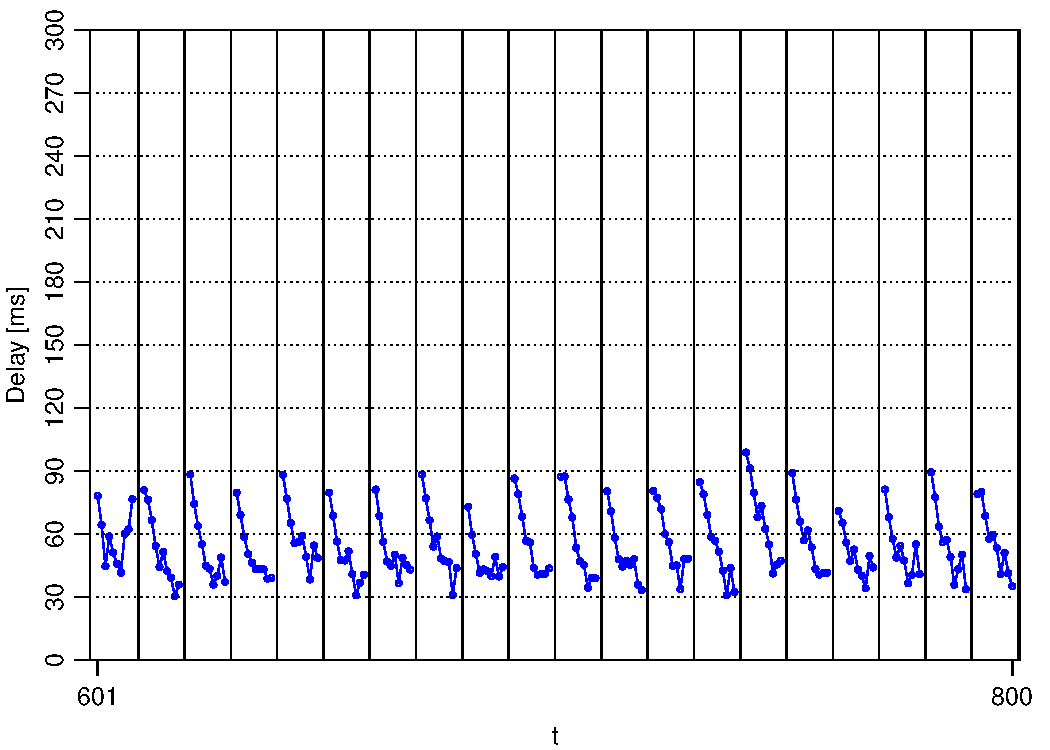
\includegraphics[width=0.33\hsize]{15-20.pdf}
}~
\subfigure[$20 \sim 25$分後]{
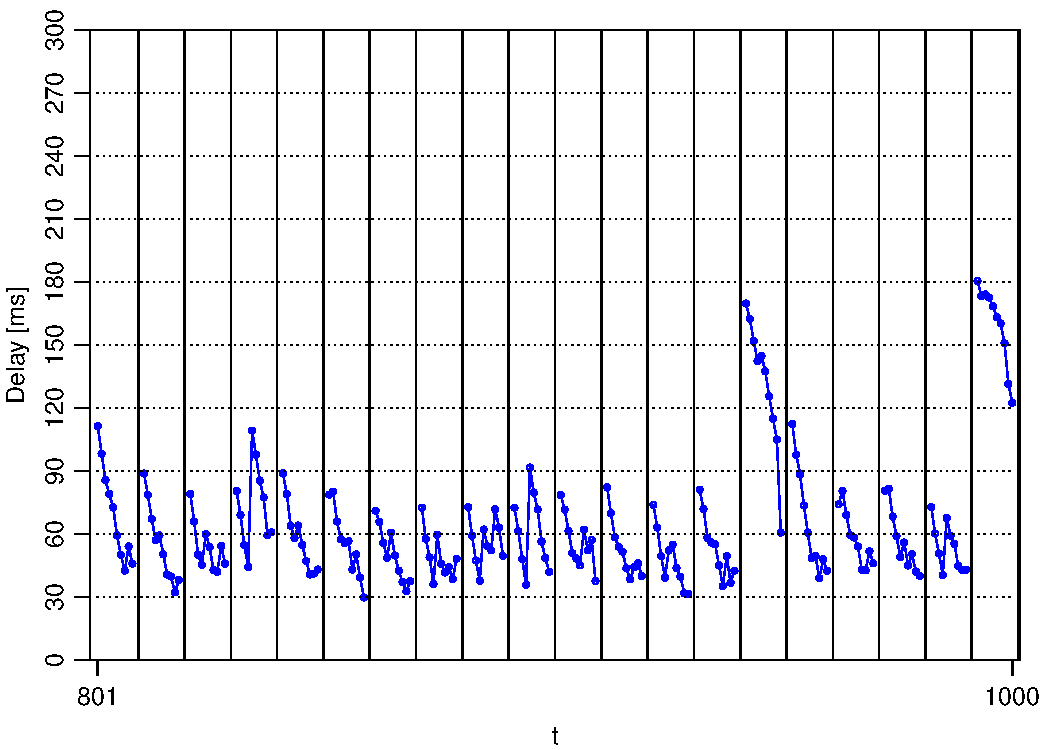
\includegraphics[width=0.33\hsize]{20-25.pdf}
}~
\subfigure[$25 \sim 30$分後]{
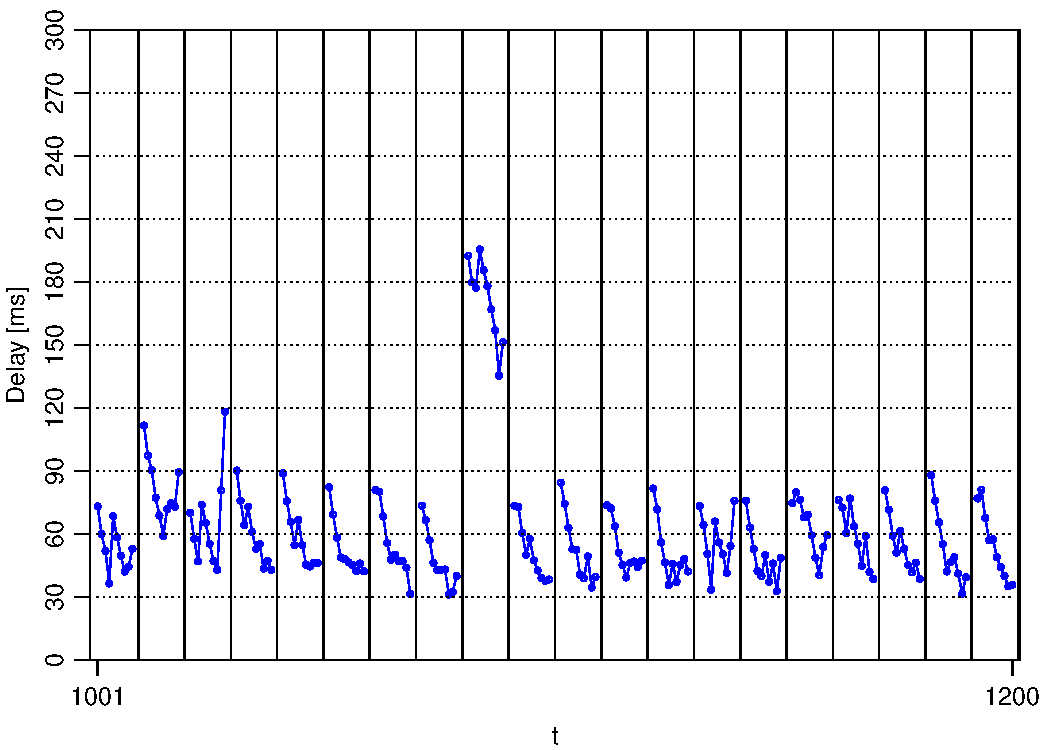
\includegraphics[width=0.33\hsize]{25-30.pdf}
}\\
\subfigure[$30 \sim 35$分後]{
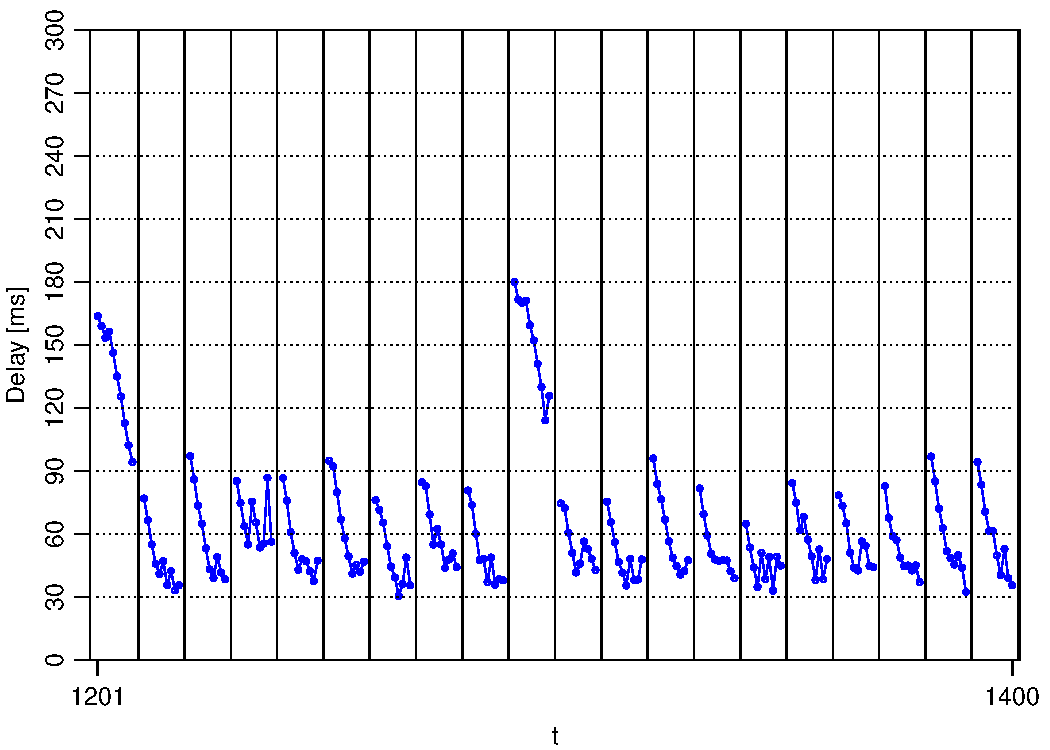
\includegraphics[width=0.33\hsize]{30-35.pdf}
}~
\subfigure[$35 \sim 40$分後]{
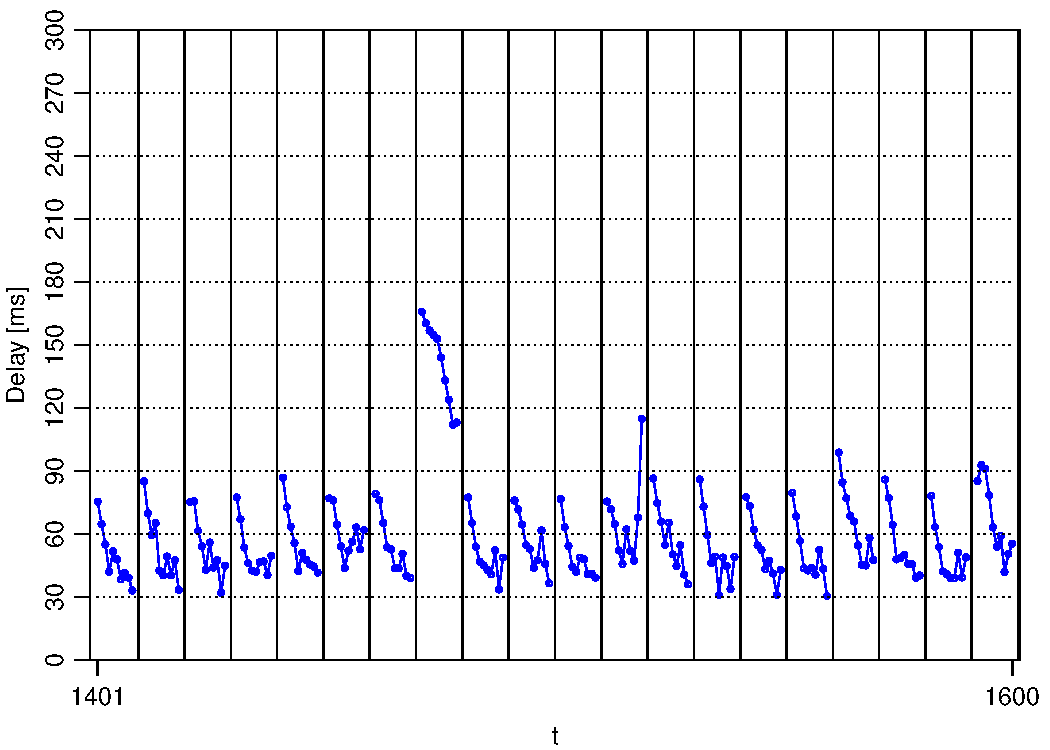
\includegraphics[width=0.33\hsize]{35-40.pdf}
}~
\subfigure[$40 \sim 45$分後]{
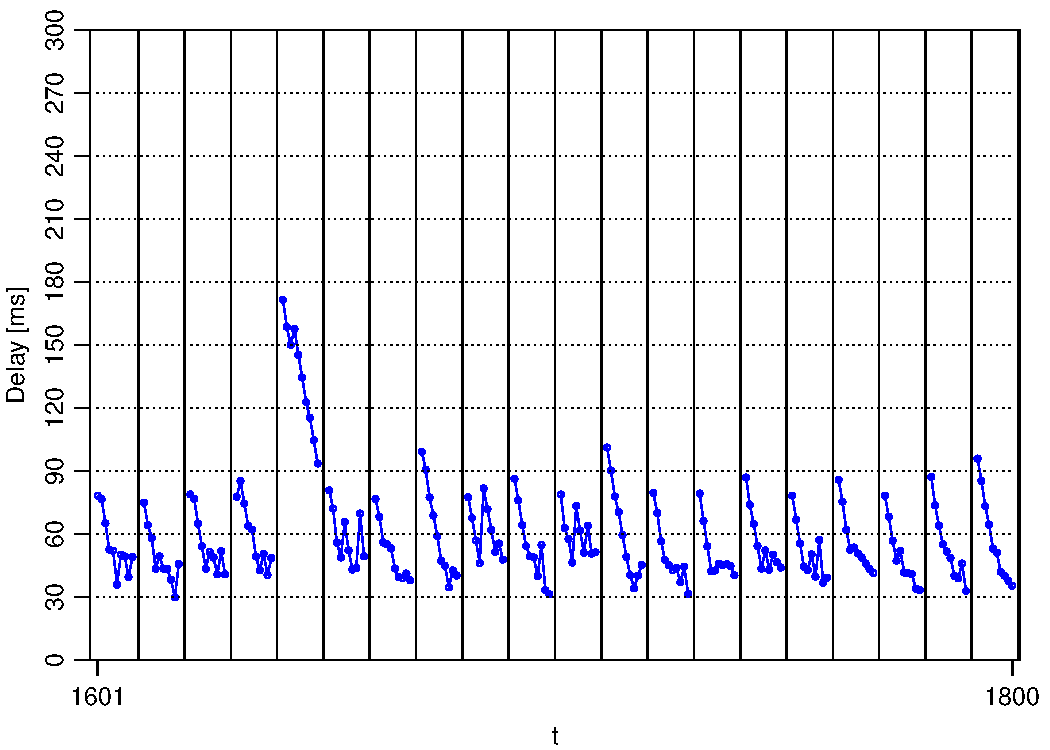
\includegraphics[width=0.33\hsize]{40-45.pdf}
}\\
\subfigure[$45 \sim 50$分後]{
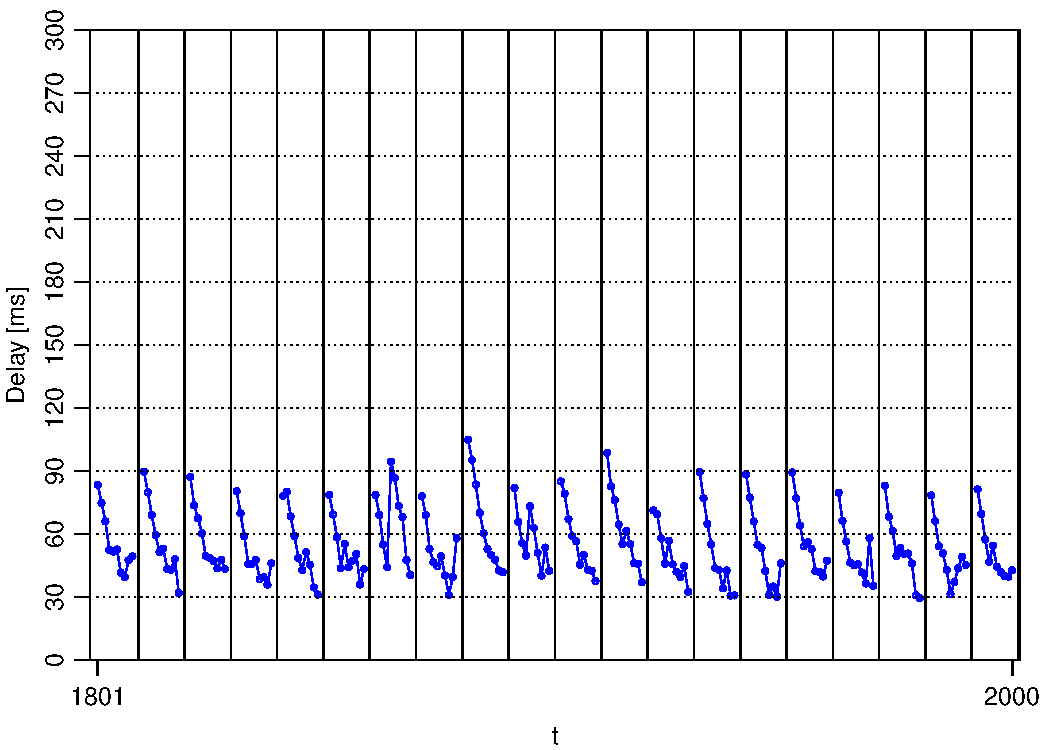
\includegraphics[width=0.33\hsize]{45-50.pdf}
}~
\subfigure[$50 \sim 55$分後]{
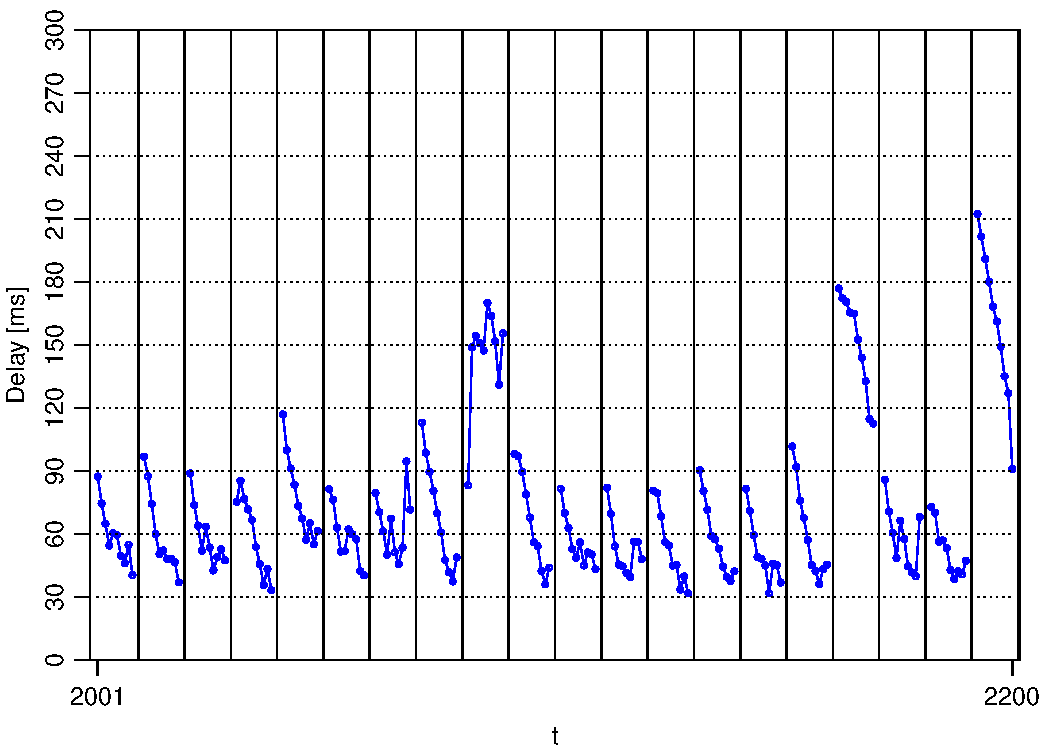
\includegraphics[width=0.33\hsize]{50-55.pdf}
}~
\subfigure[$55 \sim 60$分後]{
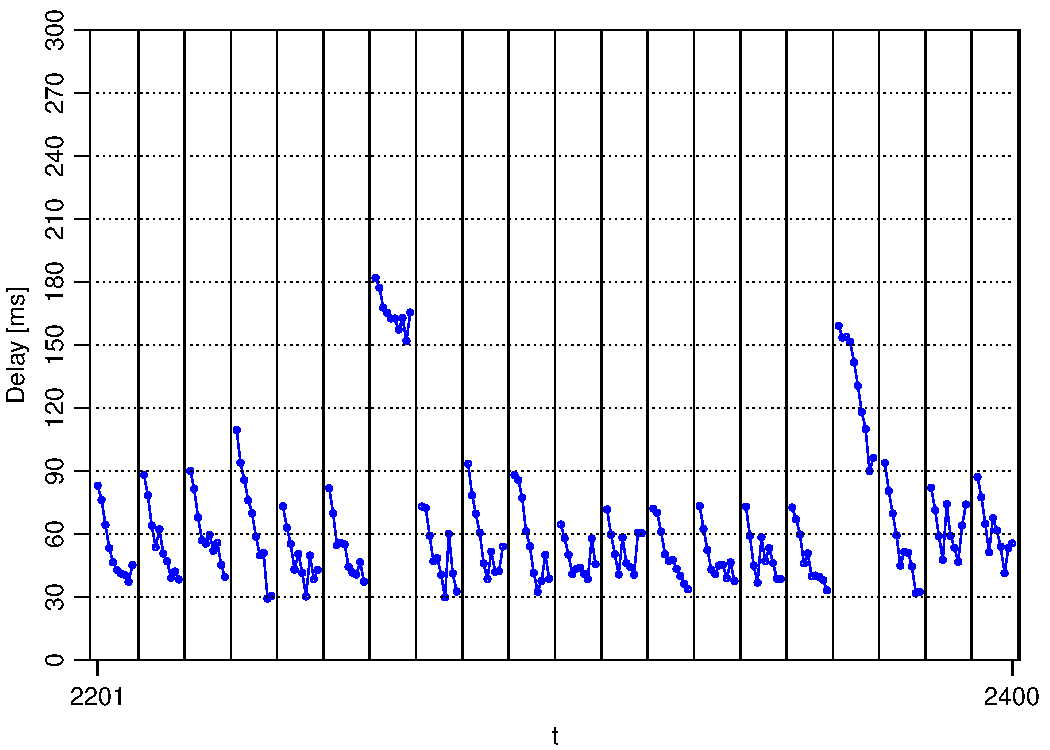
\includegraphics[width=0.33\hsize]{55-60.pdf}
}
\caption{15 秒毎の 10 ミリ秒間隔の応答遅延(計測開始から一時間経過後まで)}
\label{1}
\end{center}
\end{figure}
\begin{figure}[tb]
\begin{center}
\subfigure[$60 \sim 65$分後]{
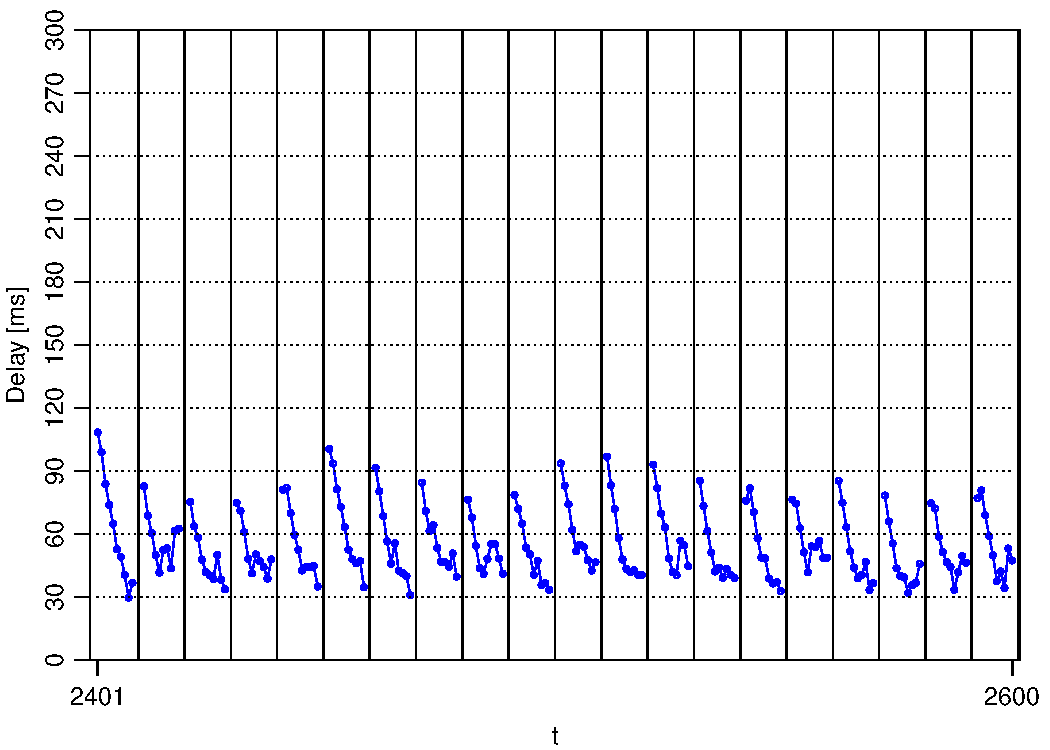
\includegraphics[width=0.33\hsize]{60-65.pdf}
}~
\subfigure[$65 \sim 70$分後]{
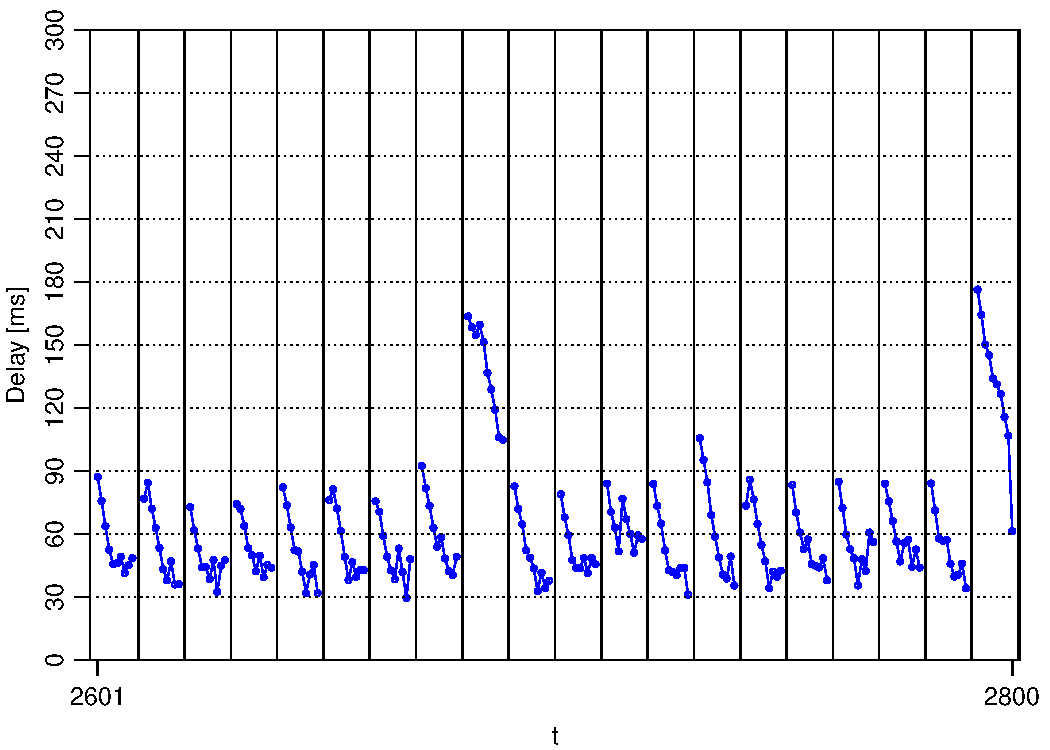
\includegraphics[width=0.33\hsize]{65-70.pdf}
}~
\subfigure[$70 \sim 75$分後]{
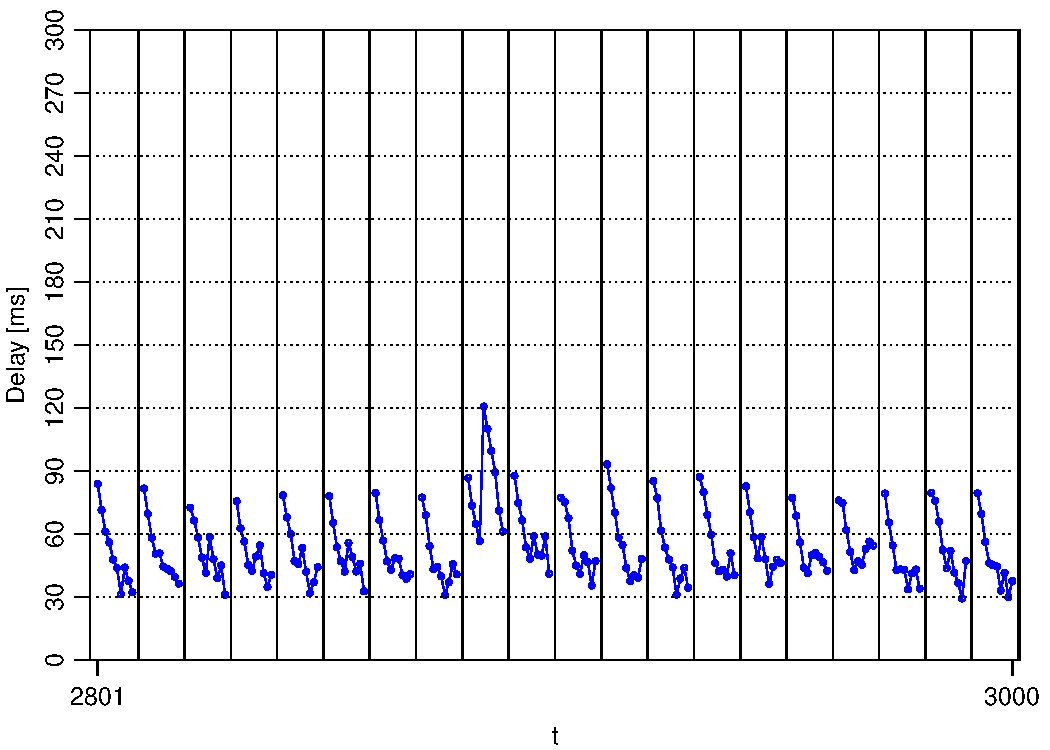
\includegraphics[width=0.33\hsize]{70-75.pdf}
}\\
\subfigure[$75 \sim 80$分後]{
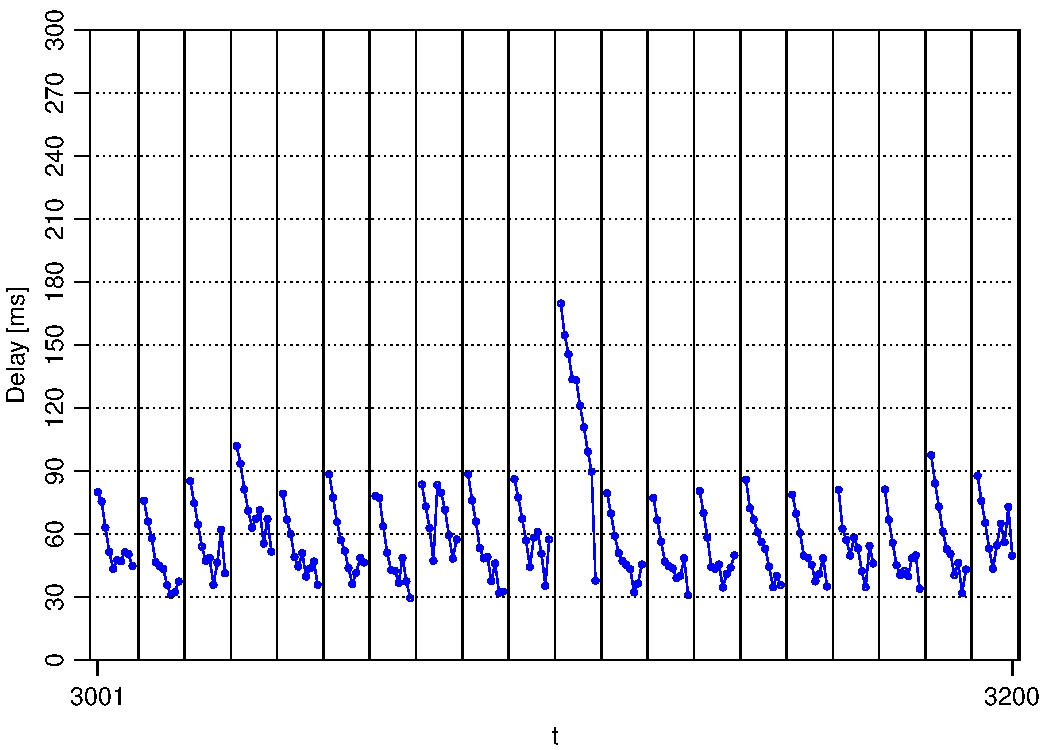
\includegraphics[width=0.33\hsize]{75-80.pdf}
}~
\subfigure[$80 \sim 85$分後]{
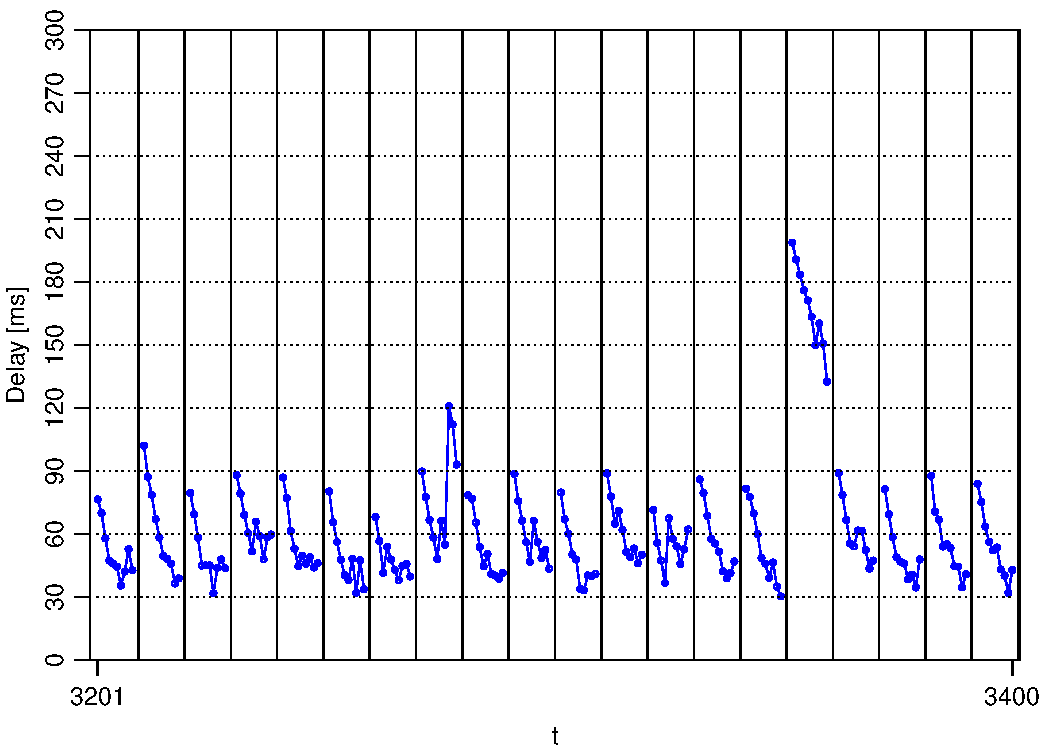
\includegraphics[width=0.33\hsize]{80-85.pdf}
}~
\subfigure[$85 \sim 90$分後]{
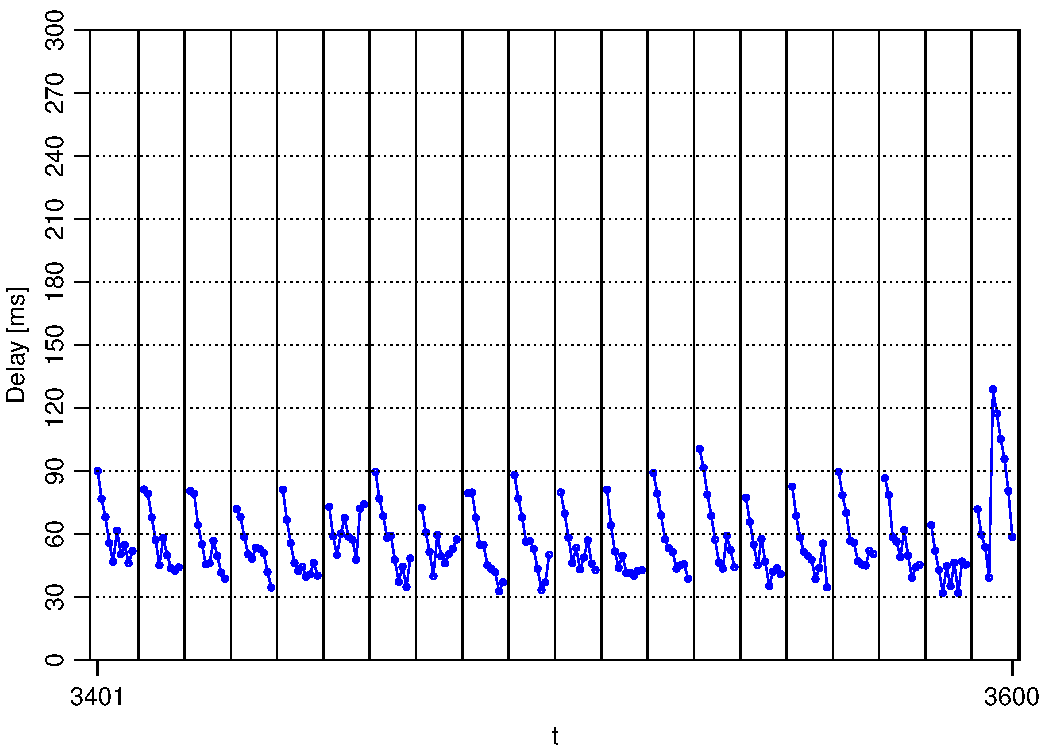
\includegraphics[width=0.33\hsize]{85-90.pdf}
}\\
\subfigure[$90 \sim 95$分後]{
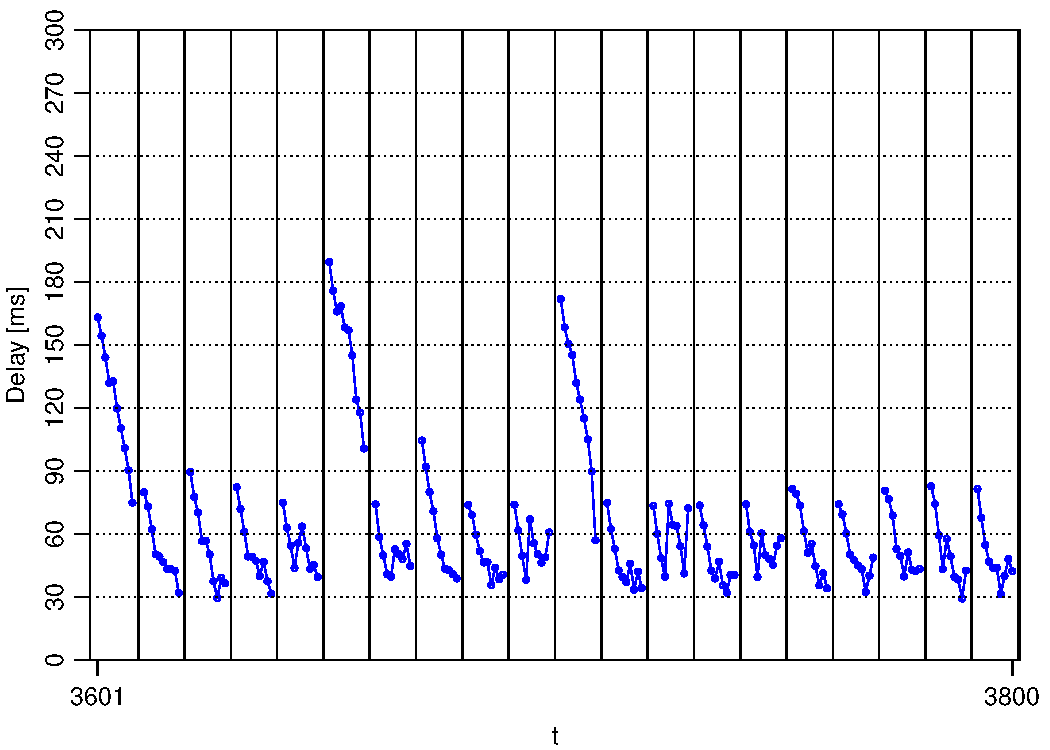
\includegraphics[width=0.33\hsize]{90-95.pdf}
}~
\subfigure[$95 \sim 100$分後]{
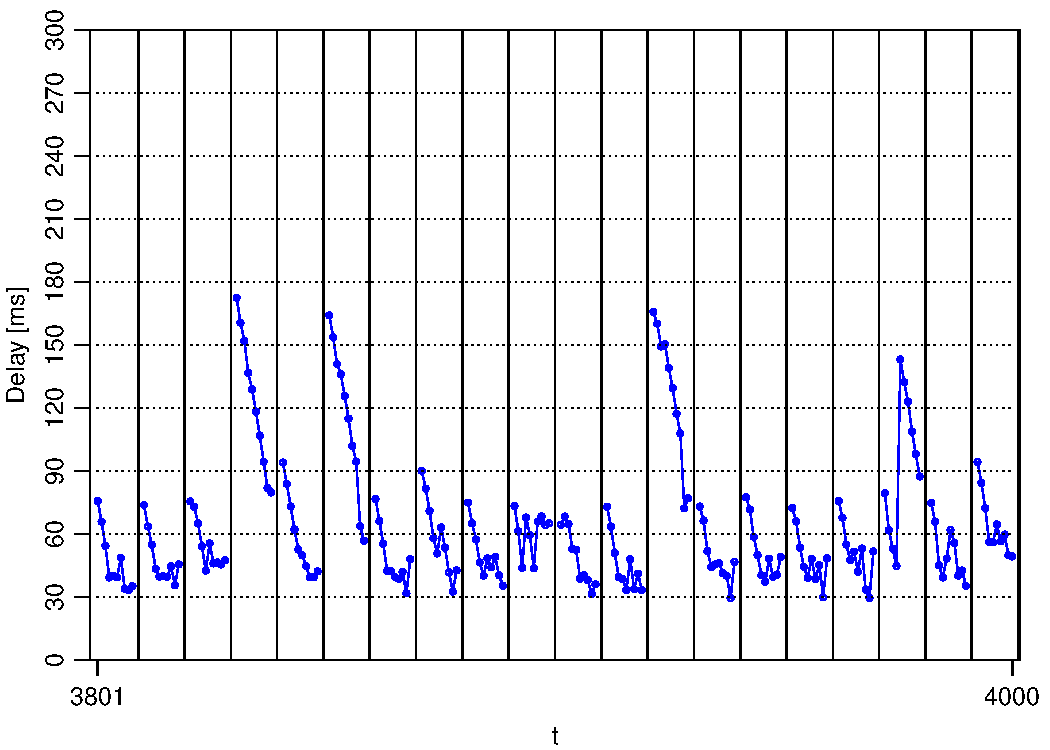
\includegraphics[width=0.33\hsize]{95-100.pdf}
}~
\subfigure[$100 \sim 105$分後]{
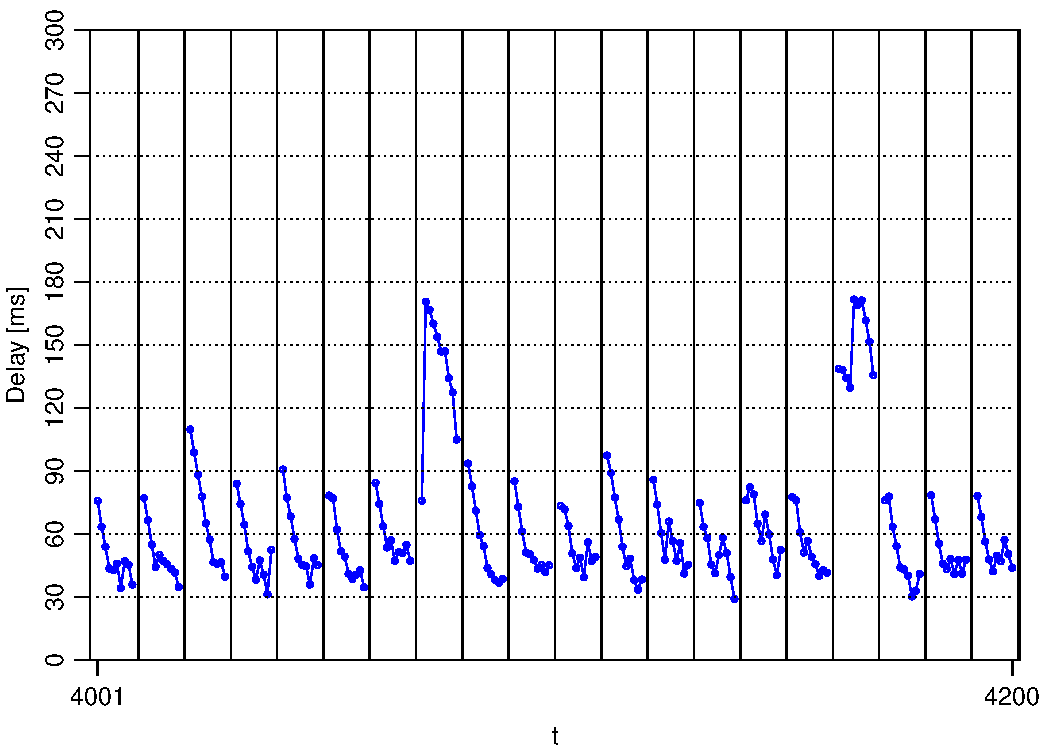
\includegraphics[width=0.33\hsize]{100-105.pdf}
}\\
\subfigure[$105 \sim 110$分後]{
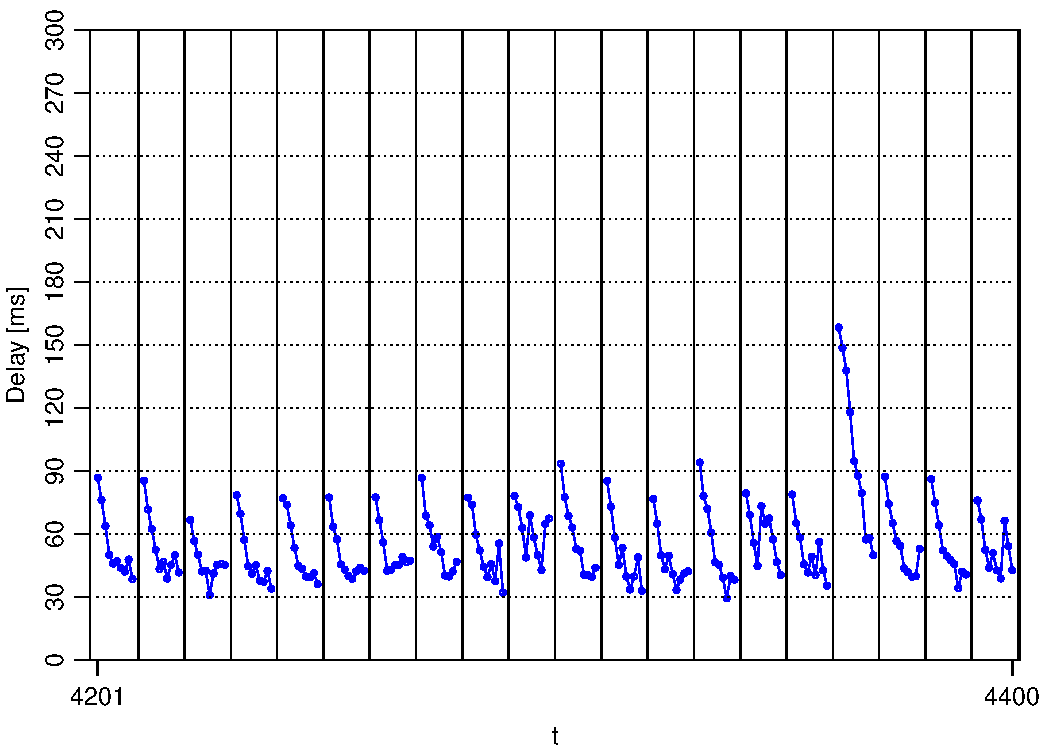
\includegraphics[width=0.33\hsize]{105-110.pdf}
}~
\subfigure[$110 \sim 115$分後]{
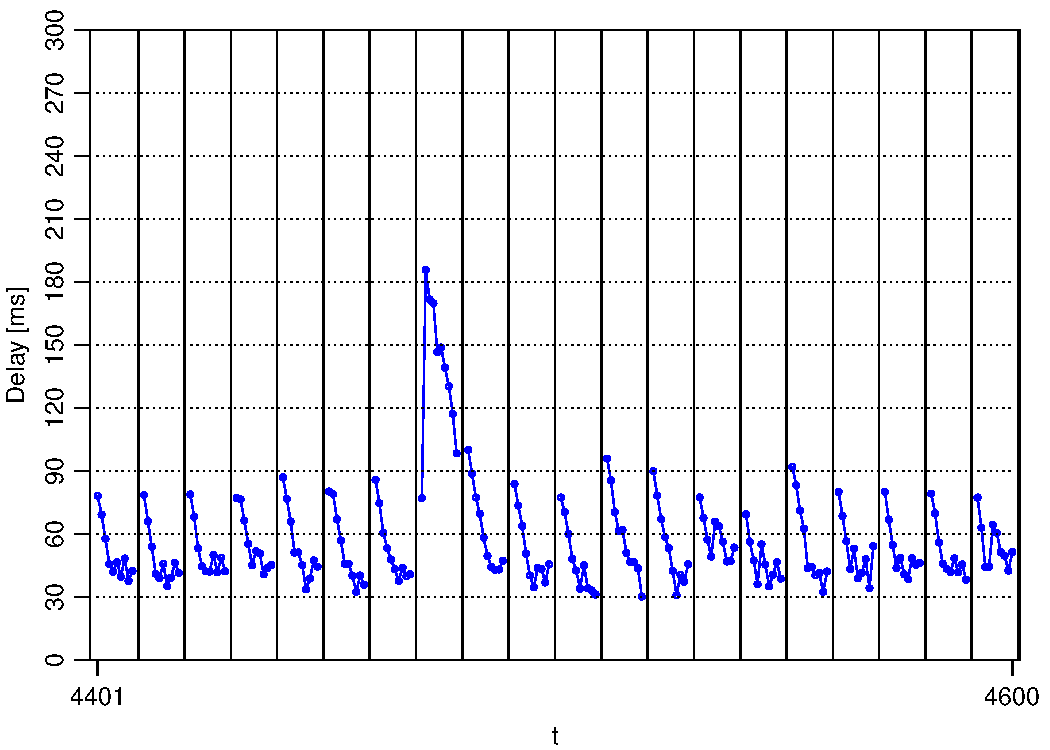
\includegraphics[width=0.33\hsize]{110-115.pdf}
}~
\subfigure[$115 \sim 120$分後]{
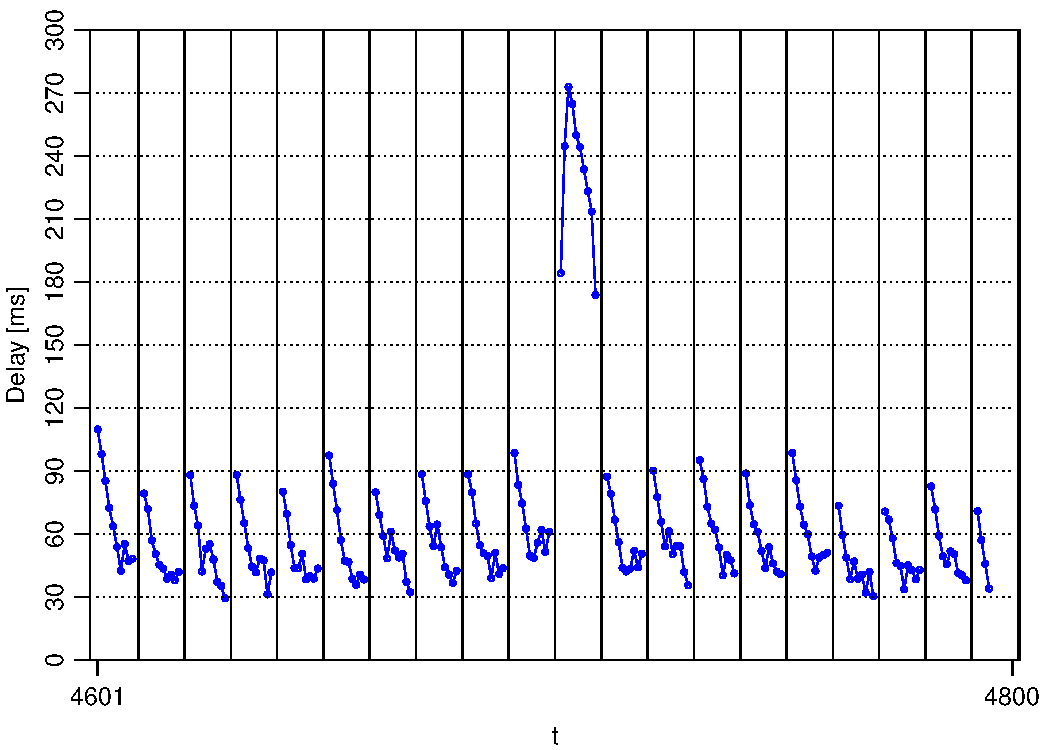
\includegraphics[width=0.33\hsize]{115-120.pdf}
}
\caption{15 秒毎の 10 ミリ秒間隔の応答遅延(一時間経過後から計測終了まで)}
\label{2}
\end{center}
\end{figure}

図より,大きな応答遅延の発生は単発的ではなく,数十ミリ秒に渡り継続して計測されることが分かった.これは例えば,図 (\ref{1}-e) の $990 \leq t \leq 1000$ や図 (\ref{1}-f) の $1080 \leq t \leq 1090$ の区間から見て取れる.
したがって,大きな値の応答遅延が計測される環境は数十ミリ程度の間続くと考えられる.ただ,実際どの程度の間継続するのかは今回の結果からは分からないため,これには追加の計測実験が必要である.

また,どの 15 秒毎の計測でも応答遅延は下降傾向にあり,最終的には 30 ms とこの計測環境においてはかなり小さな値まで下がることが分かった(後述の図 \ref{6-23} を参考).詳しいことは分からなかったが ICMP の処理系が影響していると考えられる.
\section{一日を通した計測}
今後は一日に渡った計測データの収集を行う.
これには,Raspberry Pi 上で 15 秒毎に時刻取得後に AWS サーバ(13.231.224.193)に対して ping (パケットサイズ 60 バイト, ICMP ECHO メッセージ,パケット数 1)を用いた応答遅延の計測を行うスクリプトを動かし,一分毎にこのスクリプトの起動しているかどうかを調べる.もし,起動していないようであれば計測スクリプトの再実行を行う.
図 \ref{6-23} はこのようにして得られた 6 月 23 日(火)の応答遅延データである.
横軸に時刻,縦軸に応答遅延 [ms] を取った.

\begin{figure}[tb]
\centering
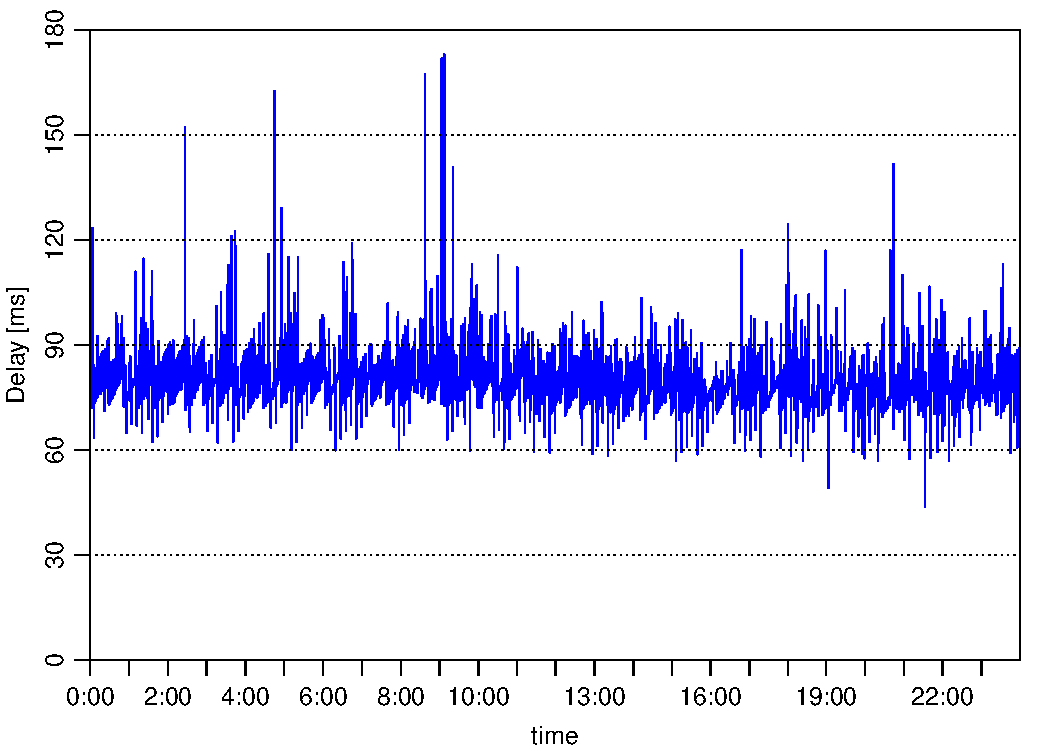
\includegraphics[width=0.9\hsize]{plot-6-23.pdf}
\caption{6 月 23 日(火)の応答遅延}
\label{6-23}
\end{figure}

図より,応答遅延は一日を通じて約 80 ms を中心に計測された.
ただ,16 時以降の応答遅延のばらつきがそれまでのものよりも大きいように思え,また,大きな応答遅延の発生頻度は 4 時台や 8 時台が高いように思える.
しかし,この単一のデータのみからは断言できないため,今後も計測を継続しこれらの分析に取り組む.

また,今までの計測データでは最小応答遅延時間が 30 ms と考えられ一時間のうちでも複数回計測されていたが,今回は 22:00 ごろに一度だけ計測された最低応答遅延時間と考えられる 35 ms はほとんど発生していないように思える.
さらに,60 ms 程度の応答遅延でも小さい方であり全体的に 70 ms から 90 ms にまとまって分布していた.
これらの差は,計測対象とするサーバの物理的な位置やネットワーク環境が異なるために生じたと考えられる.
\bibliography{myrefs}
\bibliographystyle{sieicej}
\end{document}